% Options for packages loaded elsewhere
\PassOptionsToPackage{unicode}{hyperref}
\PassOptionsToPackage{hyphens}{url}
%
\documentclass[
]{article}
\usepackage{lmodern}
\usepackage{amssymb,amsmath}
\usepackage{ifxetex,ifluatex}
\ifnum 0\ifxetex 1\fi\ifluatex 1\fi=0 % if pdftex
  \usepackage[T1]{fontenc}
  \usepackage[utf8]{inputenc}
  \usepackage{textcomp} % provide euro and other symbols
\else % if luatex or xetex
  \usepackage{unicode-math}
  \defaultfontfeatures{Scale=MatchLowercase}
  \defaultfontfeatures[\rmfamily]{Ligatures=TeX,Scale=1}
\fi
% Use upquote if available, for straight quotes in verbatim environments
\IfFileExists{upquote.sty}{\usepackage{upquote}}{}
\IfFileExists{microtype.sty}{% use microtype if available
  \usepackage[]{microtype}
  \UseMicrotypeSet[protrusion]{basicmath} % disable protrusion for tt fonts
}{}
\makeatletter
\@ifundefined{KOMAClassName}{% if non-KOMA class
  \IfFileExists{parskip.sty}{%
    \usepackage{parskip}
  }{% else
    \setlength{\parindent}{0pt}
    \setlength{\parskip}{6pt plus 2pt minus 1pt}}
}{% if KOMA class
  \KOMAoptions{parskip=half}}
\makeatother
\usepackage{xcolor}
\IfFileExists{xurl.sty}{\usepackage{xurl}}{} % add URL line breaks if available
\IfFileExists{bookmark.sty}{\usepackage{bookmark}}{\usepackage{hyperref}}
\hypersetup{
  pdftitle={gapminder plots},
  pdfauthor={Leon},
  hidelinks,
  pdfcreator={LaTeX via pandoc}}
\urlstyle{same} % disable monospaced font for URLs
\usepackage[margin=1in]{geometry}
\usepackage{color}
\usepackage{fancyvrb}
\newcommand{\VerbBar}{|}
\newcommand{\VERB}{\Verb[commandchars=\\\{\}]}
\DefineVerbatimEnvironment{Highlighting}{Verbatim}{commandchars=\\\{\}}
% Add ',fontsize=\small' for more characters per line
\usepackage{framed}
\definecolor{shadecolor}{RGB}{255,255,255}
\newenvironment{Shaded}{\begin{snugshade}}{\end{snugshade}}
\newcommand{\AlertTok}[1]{\textcolor[rgb]{0.75,0.01,0.01}{\textbf{\colorbox[rgb]{0.97,0.90,0.90}{#1}}}}
\newcommand{\AnnotationTok}[1]{\textcolor[rgb]{0.79,0.38,0.79}{#1}}
\newcommand{\AttributeTok}[1]{\textcolor[rgb]{0.00,0.34,0.68}{#1}}
\newcommand{\BaseNTok}[1]{\textcolor[rgb]{0.69,0.50,0.00}{#1}}
\newcommand{\BuiltInTok}[1]{\textcolor[rgb]{0.39,0.29,0.61}{\textbf{#1}}}
\newcommand{\CharTok}[1]{\textcolor[rgb]{0.57,0.30,0.62}{#1}}
\newcommand{\CommentTok}[1]{\textcolor[rgb]{0.54,0.53,0.53}{#1}}
\newcommand{\CommentVarTok}[1]{\textcolor[rgb]{0.00,0.58,1.00}{#1}}
\newcommand{\ConstantTok}[1]{\textcolor[rgb]{0.67,0.33,0.00}{#1}}
\newcommand{\ControlFlowTok}[1]{\textcolor[rgb]{0.12,0.11,0.11}{\textbf{#1}}}
\newcommand{\DataTypeTok}[1]{\textcolor[rgb]{0.00,0.34,0.68}{#1}}
\newcommand{\DecValTok}[1]{\textcolor[rgb]{0.69,0.50,0.00}{#1}}
\newcommand{\DocumentationTok}[1]{\textcolor[rgb]{0.38,0.47,0.50}{#1}}
\newcommand{\ErrorTok}[1]{\textcolor[rgb]{0.75,0.01,0.01}{\underline{#1}}}
\newcommand{\ExtensionTok}[1]{\textcolor[rgb]{0.00,0.58,1.00}{\textbf{#1}}}
\newcommand{\FloatTok}[1]{\textcolor[rgb]{0.69,0.50,0.00}{#1}}
\newcommand{\FunctionTok}[1]{\textcolor[rgb]{0.39,0.29,0.61}{#1}}
\newcommand{\ImportTok}[1]{\textcolor[rgb]{1.00,0.33,0.00}{#1}}
\newcommand{\InformationTok}[1]{\textcolor[rgb]{0.69,0.50,0.00}{#1}}
\newcommand{\KeywordTok}[1]{\textcolor[rgb]{0.12,0.11,0.11}{\textbf{#1}}}
\newcommand{\NormalTok}[1]{\textcolor[rgb]{0.12,0.11,0.11}{#1}}
\newcommand{\OperatorTok}[1]{\textcolor[rgb]{0.12,0.11,0.11}{#1}}
\newcommand{\OtherTok}[1]{\textcolor[rgb]{0.00,0.43,0.16}{#1}}
\newcommand{\PreprocessorTok}[1]{\textcolor[rgb]{0.00,0.43,0.16}{#1}}
\newcommand{\RegionMarkerTok}[1]{\textcolor[rgb]{0.00,0.34,0.68}{\colorbox[rgb]{0.88,0.91,0.97}{#1}}}
\newcommand{\SpecialCharTok}[1]{\textcolor[rgb]{0.24,0.68,0.91}{#1}}
\newcommand{\SpecialStringTok}[1]{\textcolor[rgb]{1.00,0.33,0.00}{#1}}
\newcommand{\StringTok}[1]{\textcolor[rgb]{0.75,0.01,0.01}{#1}}
\newcommand{\VariableTok}[1]{\textcolor[rgb]{0.00,0.34,0.68}{#1}}
\newcommand{\VerbatimStringTok}[1]{\textcolor[rgb]{0.75,0.01,0.01}{#1}}
\newcommand{\WarningTok}[1]{\textcolor[rgb]{0.75,0.01,0.01}{#1}}
\usepackage{graphicx}
\makeatletter
\def\maxwidth{\ifdim\Gin@nat@width>\linewidth\linewidth\else\Gin@nat@width\fi}
\def\maxheight{\ifdim\Gin@nat@height>\textheight\textheight\else\Gin@nat@height\fi}
\makeatother
% Scale images if necessary, so that they will not overflow the page
% margins by default, and it is still possible to overwrite the defaults
% using explicit options in \includegraphics[width, height, ...]{}
\setkeys{Gin}{width=\maxwidth,height=\maxheight,keepaspectratio}
% Set default figure placement to htbp
\makeatletter
\def\fps@figure{htbp}
\makeatother
\setlength{\emergencystretch}{3em} % prevent overfull lines
\providecommand{\tightlist}{%
  \setlength{\itemsep}{0pt}\setlength{\parskip}{0pt}}
\setcounter{secnumdepth}{5}

\title{gapminder plots}
\author{Leon}
\date{2021}

\begin{document}
\maketitle

{
\setcounter{tocdepth}{2}
\tableofcontents
}
\hypertarget{abstract}{%
\section*{Abstract}\label{abstract}}
\addcontentsline{toc}{section}{Abstract}

Statisticians and analysts have been using R (Ihaka, 1998) for a long
time. R programming environment has it's formal document standards
embedded such as R markdown. While R markdown generate documents itself
programmatically, it requires the programmer to manually construct the
structure of a file as a whole reproducible document. For the majority
of coding work done as prose contents, namely computational components,
the output are the main interest. The \textbf{listdown} Package
(Kane,Jiang and Urbanek, 2020) available on the \textbf{Comprehensive R
Archive Network (CRAN)} provides a programmatic solution to generate
documents containing computational and narrative components efficiently,
including computational components of data visualizations. However, as
the demand for big data visualizations increase rapidly in the past
decades, the capable tools for these tasks such as package
\textbf{trelliscopejs} (Hafen, Gosink, McDermott, Rodland, Kleese-Van
Dam and Cleveland, 2013) is not natively supported in high efficient
workflows of \textbf{listdown}. This paper demonstrates multiple methods
implanting interactive plotting systems and graphical packages in R to a
output document when users generate reproducible documents using the
listdown Package. These methods are mainly supported by the
\textbf{plotly} (Sievert, 2020) and \textbf{trelliscopeJS} packages
available on CRAN. The concepts are illustrated using the gapminder data
set from the \textbf{gapminder} package (Bryan, 2017), and will be
applied to a current analytical task on COVID-19 data sourced from the
World Health Organization (\url{https://www.who.int}).

\emph{Keywords: reproducible documents, effective visualizations, big
data visualizations}

\hypertarget{introduction}{%
\section{Introduction}\label{introduction}}

\hypertarget{overview}{%
\subsection{Overview}\label{overview}}

R language has been a popular computing language since its first
appearance back in the 90s (Ihaka \& Gentleman, 1996). R has many
features dedicated but not limited to statistical computing, data
analysis and other relevant tasks across a greater number of industries
and fields. In addition to the IDE (Integrated Development Environment)
software R studio, a large number of R packages are also available,
intended for users to focus more on the ``goal'' instead of the
``coding''. The paper discusses how reproducibility and compatibility of
multiple statistical tasks can be contained in one single document using
high efficient workflows, followed by data visualizations in R. While
big data visualization tasks has become much more achievable in R with
the release of many famous visualization packages such as
\textbf{trelliscopeJS} (Hafen, Gosink, McDermott, Rodland, Kleese-Van
Dam and Cleveland, 2013), listdown does not have native support for it
so far. The goal is to embed the features of these packages into
listdown, especially the idea of facetting. The result is a powerful big
data visualization tool with high efficiency workflows. All of these can
be achieved by creating \textbf{decorators} for the \textbf{listdown}
package (Kane,Jiang and Urbanek, 2020). Finally, an application of the
methods created will be demonstrated on the current COVID-19 pandemic
data sets sourced from the World Health Organization
(\url{https://www.who.int}).

\hypertarget{r-markdown}{%
\subsection{R markdown}\label{r-markdown}}

The R markdown (Baumer, Cetinkaya-Rundel, Bray, Loi, and Horton, 2014)
demonstrates the possibility of constructing reproducible documents
using R language. This format allows author to integrate R codes,
written work, data tables, visualization plots and much more information
into one directly structured document. Among scientific writings and
analytical reports knitted using R markdown, the majority are made up of
codes and narrative writings. The codes are usually but not limited to
common computing languages, such as R, Python, SQL and others. Usually
inserted between the codes, authors include contexts which explain the
code chunk itself or the output from the code chunks. Sometimes
descriptive writings are also placed between the codes using a hash, and
is usually comments of the code lines. In this paper, the chunk of
computing codes that produces outputs and the narrative writings that
describes the outputs will be referred to computational components and
narrative components respectively (Kane,Jiang and Urbanek, 2020).

Statistical analysis tends to be more reachable and interpretable to
public audience accompanied by the rapid rise of computing abilities.
While the statistical computing threshold drops with the invention of R
language, the needs to integrate computationally derived objects with
narrative explanations arise. The usage of R markdown centralizes
different data types with a specific format, further process with the
technical work in a computationally organized way. Usually in most data
analyzing tasks, the first thing is data cleaning and tidying. However,
this processes usually requires other environments and configuration to
manipulate. Such steps have different needs in computational purpose
than report or presentations. It may not be fully shown using R code or
other languages natively supported by R, but authors often use narrative
texts to describe the associate processes. These narrative texts can be
fully embedded in the R markdown file for readers to follow without
opening other documents. Before a highly informative presentation,
multiple explanatory analyses are often carried out. These explanatory
analyses contain numerous amounts of table, plots and graphs, most of
them have comments and notes. R markdown can save the robust components
and generate documents without spending time on layouts and formats.

The advantage of R markdown's narrative feature can be shown in multiple
prospects. Firstly, R markdown is as described in its name, a Markdown
syntaxed mark-up language of R. By using combinations of codes and
embedding symbols to control the formatting and layout of a R object
file, users get the desired final output document. All of these are easy
to achieve without extensive skills in coding and consume less time and
effort to learn. Packages such as bookdown (Xie, 2016) demonstrates the
easiness for users intending to edit long narrative components in
contrast of using another commonly-used markup language -- Latex. While
latex may be more expressive in terms of proficiency for academical
writing, the coding alike syntax required to produce documents takes a
substantial amount of time and effort to learn and is relatively more
complicated than R markdown's syntax. On the other hand, statistical
reports and presentations often contains numerous computational and
narrative components. R markdown supports multiple file formats once a R
object is completed and ready for publication. The function in R
markdown for this objective is called ``knit''. The process includes
running all computational components, then formatting the outputs along
with the narrative components.

In R markdown, each computational component starts with three backwards
apostrophes, with the language name and the code chunk options between
the curly brackets shall be enclosed by three backwards apostrophes
correspondingly. During the knitting process, computation components
along with their results are laid out precedingly. Each narrative
component, which is so called ordinary text with out code is combined
within the computational components, resulting in a desired file. The
final result is also customizable not only as in pdf or HTML format, but
also includes editable formats such as Microsoft word documents. This
conforms with the intention for a typical statistical report or
presentation, that is, to make audience understand statistics with less
to no statistical knowledge (Baumer, Cetinkaya-Rundel, Bray, Loi, and
Horton, 2014). R markdown fulfills this concept by offering modifiable
documents for collaborators and other users to develop narrative
components based on the statistical analysis results generated
beforehand.

While PDF and Word formats are commonly used by researchers in the
fields for their formatting specification, they do not provide a
pragmatical solution for interactive plots and graphics. Compared to
static graphics, interactive graphics are extremely powerful for
explanatory analysis, and complements the visualization prospect of
statistical visualizations (Theus \& Urbanek, 2008). Interactive
graphics not only enhances the overall aesthetics of a visualization
component, but could also reveal un-spotted insights. The findings may
change conclusions and affect the narrative components, further changing
the conclusion of a work (Healy,2018). Moreover, interactive
visualization potentially provides a solution to readers with visual
perception diseases such as color blindness (Wilke, 2019). HTML, another
format producible by R markdown, is often underestimated in its ability
for interactive visualization and animations. R has a variety of
packages that supports interactive widgets which can by knitted and
shown on HTML webpages. Despite the numerous packages and functions
supported by R to create an interactive visualization, most of them
requires an increase of workload in the computational components. A
optimal solution of merging computational components that produce
interactive graphics and the associated narrative components can be
achieved by using the decorator function in listdown package (Kane,Jiang
and Urbanek, 2020). The decorator pattern (Gamma, Helm, Johnson,
Vlissides and Patterns, 1995) in the listdown function takes elements as
arguments and returns the required object used for presentation in the
specified output directory. When it comes to visualization components
(ie. trelliscope), the plot is often fixed to a specific form
pre-defined in the computation component. The goal is to make it live
and interactive. This is possible by making use of the decorator
function in listdown.

\hypertarget{visualizations}{%
\subsection{Visualizations}\label{visualizations}}

The tools for presenting an interactive visualization was introduced
previously. The remaining problem or perhaps one of the major
limitations in creating an effective interactive plot may be the big
data sets most statistical tasks come across with nowadays (Ali, Gupta,
Nayak and Lenka, 2016). The explosive growth of data becomes a trend and
is still expanding fast accompanied by multiple factors such as the
popularization 5G and IoT (Internet of Things). Statistical
presentations and reports requiring visualizations on big data sets
becomes more challenging and creative. Interactive graphics provides an
ultimate solution, increasing the display power compared to a static
plot (Weissgerber, Garovic, Savic, Winham and Milic, 2016). Among the
various techniques on big data visualization problems, the principle of
subsetting a large data set into multiple smaller ones and presenting
them in parallel are adapted by many solutions, including the famous
\textbf{ggplot2} package (Wickham, 2011) that most R markdown users are
familiar with. The idea of Trelliscope displays (Becker, Cleveland \&
Shyu, 1996) provided a framework on multipanel graphics, and
demonstrated its huge potential in big data visualizations. However, it
was not until package \textbf{TrelliscopeJS} (Hafen, Gosink, McDermott,
Rodland, Kleese-Van Dam and Cleveland, 2013) made the interactivity of
trelliscope display possible, and further enhanced the idea by
implanting interactive functions to ggplot items, the interface is
especially effective for data with multiple categorical responses. In
this paper, multiple graphical computational components are created
using the above mentioned packages, but we will start with simple
examples such as the \textbf{plotly} package (Sievert, 2020), which
turns static ggplot objects into interactive plots. The strength and
weakness of each method, along with solutions on improving the functions
effectively for their usage in the listdown package are then followed
with examples.

The remainder of this paper will go through as follows. The next chapter
explains the motivaion of the listdown package and workflow on how the
listdown generates documents from scratch. This is a background
literature review summoning the previous work done by the package's
developers (Kane,Jiang and Urbanek, 2020) using real world COVID
-19data. This chapter also introduced the background of the data as it
is used later on. Chapter 3 discussed the implementation of decorators
using the same data from chapter 2, along with an executive summary on
the graphical outputs. Chapter 4 focused on solving more complicated
visualizations by writing functions to the decorator of the listdown
package. Chapter 5 applied the mechanisms to the COVID-19 data, and
revealed the relationship of new cases and death number of each country
by a specific time frame. The final chapter discussed the results of the
output, concluded the limitations and further work.

\hypertarget{package-listdown}{%
\section{Package Listdown}\label{package-listdown}}

\hypertarget{high-efficiency-workflows}{%
\subsection{High Efficiency Workflows}\label{high-efficiency-workflows}}

Lets suppose the data analyzing part and all coding work has completed
for an analysis. The results of the analysis containing summary tables,
data tables and plots which we referred to computational components
earlier, are collected into lists of objects and saved as a RDS or RDATA
format file. They are in the order of which the author would like to
present them separately in respect to the whole analysis, the next thing
is to produce the components from the lists into a document like a html
file. This is a typical order of a data analyzing work processes, but it
is not definite. The computational components are not required to be
turned into lists, but it is often the case for R users when dealing
with multiple computational components. The objects in RDS and RDATA
format files can be restored and reproduced in R environment easily, and
has many advantages.

Sometimes, the computational components along with the results they
produce are stored in multiple locations, or in many cases, on different
machines. It is especially important to centralize them. They have
multiple properties obtained naturally when turned into lists. Firstly,
changing them into elements of a list generically provides a
hierarchical structure for centralizing. Secondly, for most data, even
on large scales, the actual presented contents are relatively small.
Storing them into lists allows easier access and aligns with the
concepts of centering. Lastly, if the elements in the list are not in
the order of a presentation desired, or changes accordingly,
manipulating the order is much more convenient than non-centralized
components. Nonetheless, the data cleaning and other processes
iteratively repeats each time generating documents for presentation
whenever knitr is used in a R markdown file. A R markdown file generally
lacks semantic structure. When all computational components and
narrative components are stored in one single file manually paragraphed
by the author, extracting and editing components partially in a R
markdown file often leads to increase of workloads after the changes are
committed.

During a statistical analysis, the analytical process and results can be
seen as two parts which can be stored separately. If the results contain
graphs and plots, they could be further stored in single named lists. As
everything is organized in named lists, listdown has several advantages
compared to normal R markdown files containing all computational and
narrative components. First, it allows multiple pathways working in
parallel from the same data. When the experiment and objective is
different based on the same data set, computational components are
expected to be different. This will affect the narrative components such
as contexts and discussions, but the data set along with other processes
such as cleaning and tidying remains constant. Since the different
``pathways'' can be stored into different lists, listdown package allows
users to selectively pick the reproducible lists along with the
narrative components. R markdown files shows the experiment in a serial
way if different analyses from the same data are stored in the same
file, or users will have to open two R markdown files with the same
computational component for processing in both R markdown files.

In addition, R markdown does not hold any data dedicated for the file
itself. In order for a computational component in R markdown that reads
in the data to work, the data set has to be stored or set to a pathway
specifying the location of the data, depending on either it is saved
locally or on a server.

To overcome the above mentioned aspects, package listdown (Kane,Jiang
and Urbanek, 2020) was introduced providing functions to
programmatically create R markdown files from named lists. By using
functions from the package, the components can be turned into a single
named list, organized in a hierarchical structure. The contents of each
list denoted, including the name and type of R object can be viewed in
dendrograms. On top of the lists, decorators and other customizable
functions can be added to assist the problem of visualizing. This is
particular useful when large datasets are added to its corresponding
computational component list and the author intends to present them.
Large data sets requires a substantial amount of space to be fully
shown.

Another advantage for using the listdown package is its capability to
avoid repetitive work when data analysis updates. This is partially
useful when data analysis process is updated frequently while the data
source remains in the same format and standard. Once the computational
components for data cleaning and process are constructed and stored into
the list, the analysis may change the output such as results and plots.
It may further change the narrative components. However, updating
analysis methods does not mean deprecating the previous methods,
listdown package allows different workflows and pathways to be stored
and reproduced at anytime with knitr, this vastly improves efficiency
and drops tedious repetitive works while maintaining the objectives
desired. Some useful areas of statistical analysis benefiting from the
listdown package are mainly but not limited to its usage in clinical
trial and medical data (Kane,Jiang and Urbanek, 2020). The final case
study verifies this statement.

\hypertarget{listdown-working-steps}{%
\subsection{Listdown Working Steps}\label{listdown-working-steps}}

The workflow for users using the listdown package are described as the
follows:

\begin{enumerate}
\def\labelenumi{\arabic{enumi}.}
\item
  The computational components in R are turned into list of objects,
  Each computational components are named, and is part of the named
  list.
\item
  The named list containing all computational components are saved to
  the current directory on the disk as \emph{RDS} or \emph{RDATA}
  formatted files.
\item
  By using function \textbf{listdown()}, the RDS is then read into R as
  a listdown class object. At this step, multiple components are added.
  First, the required package for the current listdown object to run are
  specified. Second, the decorator arguments are described. Third,
  initial expressions that runs before the listdown object knits are
  stated . Lastly, the document wide R chunk options are added in.
\item
  The header is then added, including the title of the output document,
  the author and the date. This is an optional step, and is not
  necessary in the workflow steps, however, it would be sensible to add
  the title in for readers to understand better.
\item
  The listdown object with the header are now sufficient to create a
  document, functions \textbf{writeLines} from package knitr (Xie, 2013)
  turns the listdown object to a R markdown file ready for rendering.
\item
  The last step is to render the R markdown file to a output document.
  For the purpose of this paper, HTML format is ideal for all
  interactive plots and graphics. The R markdown is turned into markdown
  from knitr, the functions added in the listdown object at step 3 such
  as decorators and initial expressions injects through the kntting
  process, and produces the final HTML output. For the next part, the
  above steps will be explained in detail using a real world example
  data set.
\end{enumerate}

\hypertarget{case-study-covid-19-dataset-example}{%
\subsection{Case Study: COVID-19 Dataset
Example}\label{case-study-covid-19-dataset-example}}

The data set regions from the \textbf{COVID-regions-2021.csv} file (
World Health Organization, 2021) is used in this first example. In this
data set, 4 key information are contained. Firstly, all the WHO
membership countries around the globe are grouped spatially and
culturally according to the World Health Organization into regions. The
six big WHO regions are:

\begin{itemize}
\item
  African Region
\item
  Region of the Americas
\item
  South-East Asia Region
\item
  European Region
\item
  Eastern Mediterranean Region
\item
  Western Pacific Region
\end{itemize}

These regions are shown in each of their corresponding abbreviations
under the variable \emph{``WHO\_region''}. Secondly, the date
information under the \emph{Date\_reported} variable is inclusive of
2020 and the first quarter of 2021. To be more exact, from 3rd of
January 2020 to the 15th of March 2021. Thirdly, The number of new cases
and the number of new deaths for each day of the regions has been
included and named \emph{New\_cases} and \emph{New\_deaths}. Four
visualization objects produced using \textbf{ggplot2} (Wickham, 2011)
were saved in RDS formatted file as a list named
\emph{``computational\_components\_covid''}. The objects are named ``New
cases per day for each region'', ``New cases per day for each region
facet'', ``Cases against Death'' and ``Cases against Death facet'', each
containing their corresponding graphics. The first two plots used
\textbf{geom\_area()} to show the number of new cases recorded each day
for all the regions in the given time frame. While the third and fourth
plot shows the relationship of new cases against death recorded by day,
and is plotted with \textbf{geom\_point()}. The main difference within
the first and second plot, the third and the fourth plot, is the
additional function call \textbf{facet\_wrap()} in the ggplot function.
In the facet\_wrap arguments, a variable must be defined, such that the
original data is separately plotted in respect to the defined variable
of the argument. This function allows each panel in the plot to show a
subset or a proportion of the data, and has advantage in comparing
patterns and trends. The function works well especially in the situation
where there are severely overlapping data points, or when there are too
much (but not over numbered) levels in the defined variable. Later in
this paper, we will discuss advanced solutions to big data sets with
multiple levels that needs to be visualized effectively.

Once data has been read into R, the computational component is
reproduced and stored along with the data into a named list, in this
case, it is called \emph{``comp\_covid''}. It is then saved to the
current directory as a R object.

\hypertarget{making-a-list-of-computational-components}{%
\subsubsection{Making a list of Computational
Components}\label{making-a-list-of-computational-components}}

\begin{Shaded}
\begin{Highlighting}[]
\CommentTok{\# Read in the regions data set.}
\NormalTok{regions =}\StringTok{ }\KeywordTok{read.csv}\NormalTok{(}\StringTok{"COVID{-}regions{-}2021.csv"}\NormalTok{, }
                    \DataTypeTok{colClasses=}\KeywordTok{c}\NormalTok{(}\StringTok{"character"}\NormalTok{, }\StringTok{"Date"}\NormalTok{, }\KeywordTok{rep}\NormalTok{(}\StringTok{"numeric"}\NormalTok{, }\DecValTok{2}\NormalTok{)))}

\CommentTok{\# Creating the computational components}
\NormalTok{computational\_components\_covid \textless{}{-}}\StringTok{ }\KeywordTok{list}\NormalTok{( }
  \StringTok{\textasciigrave{}}\DataTypeTok{New cases per day for each region}\StringTok{\textasciigrave{}}\NormalTok{ =}\StringTok{ }\KeywordTok{ggplot}\NormalTok{(regions) }\OperatorTok{+}\StringTok{ }
\StringTok{    }\KeywordTok{geom\_area}\NormalTok{(}\KeywordTok{aes}\NormalTok{(Date\_reported, New\_cases, }\DataTypeTok{colour=}\NormalTok{WHO\_region, }\DataTypeTok{fill=}\NormalTok{WHO\_region), }
              \DataTypeTok{stat=}\StringTok{"smooth"}\NormalTok{, }
              \DataTypeTok{alpha=}\NormalTok{.}\DecValTok{2}\NormalTok{, }\DataTypeTok{position=}\StringTok{"identity"}\NormalTok{,}
              \DataTypeTok{method=}\StringTok{"loess"}\NormalTok{, }\DataTypeTok{span=}\NormalTok{.}\DecValTok{1}\NormalTok{) }\OperatorTok{+}
\StringTok{    }\KeywordTok{labs}\NormalTok{(}\DataTypeTok{title =} \StringTok{"Number of daily COVID cases by WHO region"}\NormalTok{) }\OperatorTok{+}
\StringTok{    }\KeywordTok{scale\_y\_continuous}\NormalTok{(}\DataTypeTok{expand =} \KeywordTok{rep}\NormalTok{(}\DecValTok{0}\NormalTok{,}\DecValTok{4}\NormalTok{),}\DataTypeTok{labels =} \KeywordTok{label\_comma}\NormalTok{()) }\OperatorTok{+}
\StringTok{    }\KeywordTok{scale\_x\_date}\NormalTok{(}\DataTypeTok{limits =} \KeywordTok{as.Date}\NormalTok{(}\KeywordTok{c}\NormalTok{(}\StringTok{"2020{-}01{-}01"}\NormalTok{, }\StringTok{"2021{-}03{-}15"}\NormalTok{)),}
                 \DataTypeTok{expand =} \KeywordTok{expansion}\NormalTok{(}\DecValTok{0}\NormalTok{),}
                 \DataTypeTok{label =} \KeywordTok{label\_date\_short}\NormalTok{()),}

\StringTok{\textasciigrave{}}\DataTypeTok{New cases per day for each region facet}\StringTok{\textasciigrave{}}\NormalTok{ =}
\StringTok{   }\KeywordTok{ggplot}\NormalTok{(regions, }\KeywordTok{aes}\NormalTok{(}\DataTypeTok{x =}\NormalTok{ Date\_reported, }\DataTypeTok{y =}\NormalTok{ New\_cases,}
                       \DataTypeTok{col =}\NormalTok{ WHO\_region, }\DataTypeTok{fill =}\NormalTok{ WHO\_region,}
                       \DataTypeTok{stat =} \StringTok{"smooth"}\NormalTok{,  }\DataTypeTok{method=}\StringTok{"loess"}\NormalTok{, }\DataTypeTok{span=}\NormalTok{.}\DecValTok{1}\NormalTok{)) }\OperatorTok{+}
\StringTok{   }\KeywordTok{geom\_area}\NormalTok{( }\DataTypeTok{alpha=}\NormalTok{.}\DecValTok{5}\NormalTok{) }\OperatorTok{+}\StringTok{ }
\StringTok{  }\KeywordTok{facet\_wrap}\NormalTok{(.}\OperatorTok{\textasciitilde{}}\NormalTok{WHO\_region) }\OperatorTok{+}
\StringTok{  }\KeywordTok{labs}\NormalTok{(}\DataTypeTok{title =} \StringTok{"Number of daily COVID cases by WHO region facet"}\NormalTok{) }\OperatorTok{+}
\StringTok{  }\KeywordTok{scale\_y\_continuous}\NormalTok{(}\DataTypeTok{expand =} \KeywordTok{rep}\NormalTok{(}\DecValTok{0}\NormalTok{,}\DecValTok{4}\NormalTok{),}\DataTypeTok{labels =} \KeywordTok{label\_comma}\NormalTok{()) }\OperatorTok{+}
\StringTok{  }\KeywordTok{scale\_x\_date}\NormalTok{(}\DataTypeTok{limits =} \KeywordTok{as.Date}\NormalTok{(}\KeywordTok{c}\NormalTok{(}\StringTok{"2020{-}01{-}01"}\NormalTok{, }\StringTok{"2021{-}03{-}15"}\NormalTok{)),}
               \DataTypeTok{expand =} \KeywordTok{expansion}\NormalTok{(}\DecValTok{0}\NormalTok{),}
               \DataTypeTok{label =} \KeywordTok{label\_date\_short}\NormalTok{()),}

\StringTok{\textasciigrave{}}\DataTypeTok{Cases against Death}\StringTok{\textasciigrave{}}\NormalTok{ =}\StringTok{ }\KeywordTok{ggplot}\NormalTok{(}\DataTypeTok{data =}\NormalTok{ regions,}
    \KeywordTok{aes}\NormalTok{(}\DataTypeTok{x=}\NormalTok{New\_cases, }\DataTypeTok{y=}\NormalTok{New\_deaths, }\DataTypeTok{color =}\NormalTok{ WHO\_region)) }\OperatorTok{+}
\StringTok{    }\KeywordTok{geom\_point}\NormalTok{(}\DataTypeTok{alpha =} \FloatTok{.2}\NormalTok{) }\OperatorTok{+}\StringTok{ }
\StringTok{    }\KeywordTok{scale\_x\_sqrt}\NormalTok{() }\OperatorTok{+}\StringTok{ }\KeywordTok{scale\_y\_sqrt}\NormalTok{() }\OperatorTok{+}
\StringTok{    }\KeywordTok{labs}\NormalTok{(}\DataTypeTok{title =} \StringTok{"Number of COVID cases against death by WHO region"}\NormalTok{),}
     

\StringTok{\textasciigrave{}}\DataTypeTok{Cases against Death facet}\StringTok{\textasciigrave{}}\NormalTok{ =}\StringTok{ }\KeywordTok{ggplot}\NormalTok{(}\KeywordTok{filter}\NormalTok{(regions, New\_cases }\OperatorTok{\textgreater{}=}\StringTok{ }\DecValTok{0}\NormalTok{),}
    \KeywordTok{aes}\NormalTok{(New\_cases, New\_deaths, }\DataTypeTok{colour=}\NormalTok{WHO\_region)) }\OperatorTok{+}\StringTok{ }
\StringTok{    }\KeywordTok{geom\_point}\NormalTok{(}\DataTypeTok{alpha=}\NormalTok{.}\DecValTok{2}\NormalTok{) }\OperatorTok{+}
\StringTok{    }\KeywordTok{scale\_x\_sqrt}\NormalTok{() }\OperatorTok{+}\StringTok{ }\KeywordTok{scale\_y\_sqrt}\NormalTok{() }\OperatorTok{+}
\StringTok{    }\KeywordTok{facet\_wrap}\NormalTok{(}\KeywordTok{vars}\NormalTok{(WHO\_region)) }\OperatorTok{+}
\StringTok{    }\KeywordTok{theme}\NormalTok{(}\DataTypeTok{aspect.ratio=}\DecValTok{1}\NormalTok{, }\DataTypeTok{legend.position=}\StringTok{"none"}\NormalTok{) }\OperatorTok{+}
\StringTok{    }\KeywordTok{labs}\NormalTok{(}\DataTypeTok{title =} \StringTok{"Number of COVID cases against death by WHO region by facet"}\NormalTok{)}
\NormalTok{)}

\CommentTok{\#Save file to the disk}
\KeywordTok{saveRDS}\NormalTok{(computational\_components\_covid, }\StringTok{"comp{-}comp\_covid.rds"}\NormalTok{)}
 
\NormalTok{comp\_covid \textless{}{-}}\StringTok{ }\KeywordTok{readRDS}\NormalTok{(}\StringTok{"comp{-}comp\_covid.rds"}\NormalTok{)}

\KeywordTok{ld\_cc\_dendro}\NormalTok{(comp\_covid)}
\end{Highlighting}
\end{Shaded}

\begin{verbatim}
## 
## comp_covid
##   |-- New cases per day for each region
##   |  o-- object of type(s):gg ggplot
##   |-- New cases per day for each region facet
##   |  o-- object of type(s):gg ggplot
##   |-- Cases against Death
##   |  o-- object of type(s):gg ggplot
##   o-- Cases against Death facet
##      o-- object of type(s):gg ggplot
\end{verbatim}

After reading in our computational component that has been saved, the
next step is to create a listdown object. The function
\textbf{ld\_cc\_dendro()} shows each object in the listdown in an
descending order of depth (Kane,Jiang and Urbanek, 2020). Because every
object in the component is named, it is also labeled in prior to the
description of each object.

\hypertarget{creating-a-listdown-object}{%
\subsubsection{Creating a Listdown
object}\label{creating-a-listdown-object}}

From the previous step, the list containing the plots now saved as a R
object named \emph{comp-comp\_covid.rds} has the following choices for
authors to decide:

\begin{enumerate}
\def\labelenumi{\arabic{enumi}.}
\item
  A listdown object will be created using function \textbf{listdown()}.
  The object will be loaded into the designated document with a
  specified way, along with the libraries and codes required for the
  computational component. In this example, building the computational
  components in the list requires library \textbf{ggplot2},
  \textbf{tidyverse} and \textbf{scales}, hence they are specified and
  loaded together with the saved computational object.
\item
  Then the author decides how the elements in the list will be presented
  in the document by using \textbf{decorator()} function which will are
  demonstrated in the next example.
\item
  Initial expressions that gets evaluated before knitting is included
  using \textbf{init\_expr()}, this will be demonstrated later in
  chapter 3.
\item
  The chunk options can be controlled two ways. The first being normal
  chunk options, which can be specified straight away, the second is by
  using \textbf{decorator\_chunk\_opts()} , and can be subjected to a
  class given.
\end{enumerate}

\begin{verbatim}
## [1] "listdown"
\end{verbatim}

\begin{verbatim}
## 
## Listdown object description
## 
##     Package(s) imported:
##  ggplot2
##  tidyverse
##  scales
## 
##     Setup expression(s) (run before packages are loaded):
##  (none)
## 
##     Initial expression(s) (run after packages are loaded):
##  (none)
## 
##     Expression to read data:
##  readRDS("comp-comp_covid.rds")
## 
##     Decorator(s):
##  (none)
## 
##     Defaut decorator:
##  identity
## 
##     Chunk option(s):
##  (none)
## 
##     Decorator chunk option(s):
##  (none)
\end{verbatim}

From the output, we can see ld\_new is a listdown class object, the
descriptions are as shown. Here, no initial expression, decorators,
chunk options and decorator chunk options are added, the ggplot objects
will be rendered just like any normal R markdown file.

\hypertarget{header-options}{%
\subsubsection{Header Options}\label{header-options}}

The listdown object named \textbf{ld\_new} is now ready to create the
document. To regularize the document output in terms of formats, it is
further processed with a header. The listdown package has native support
in R markdown and \textbf{workflowr} as yml objects (Kane,Jiang and
Urbanek, 2020). The header objects are part of the list in the document,
and can be edited by using \texttt{ld\_rmarkdown\_header()}. By calling
the document name, a glimpse of the document content is shown, the names
are clearly listed out along with the type of objects author intends to
include. This step is optional as described in the previous working
steps, however, it is always important to include a name for the outputs
as it follows the principle of proportional ink (Wilke, 2019).

\begin{Shaded}
\begin{Highlighting}[]
\NormalTok{covidexample \textless{}{-}}
\StringTok{  }\KeywordTok{c}\NormalTok{(}\KeywordTok{as.character}\NormalTok{(}\KeywordTok{ld\_rmarkdown\_header}\NormalTok{(}\StringTok{"Covid plots"}\NormalTok{, }\DataTypeTok{author =} \StringTok{"Leon"}\NormalTok{, }\DataTypeTok{date =} \StringTok{"2021"}\NormalTok{)),}
    \KeywordTok{ld\_make\_chunks}\NormalTok{(ld\_new))}

\NormalTok{covidexample}
\end{Highlighting}
\end{Shaded}

\begin{verbatim}
##  [1] "---"                                              
##  [2] "title: Covid plots"                               
##  [3] "author: Leon"                                     
##  [4] "date: '2021'"                                     
##  [5] "output: html_document"                            
##  [6] "---"                                              
##  [7] ""                                                 
##  [8] "```{r}"                                           
##  [9] "library(ggplot2)"                                 
## [10] "library(tidyverse)"                               
## [11] "library(scales)"                                  
## [12] ""                                                 
## [13] "cc_list <- readRDS(\"comp-comp_covid.rds\")"      
## [14] "```"                                              
## [15] ""                                                 
## [16] "# New cases per day for each region"              
## [17] ""                                                 
## [18] "```{r}"                                           
## [19] "cc_list$`New cases per day for each region`"      
## [20] "```"                                              
## [21] ""                                                 
## [22] "# New cases per day for each region facet"        
## [23] ""                                                 
## [24] "```{r}"                                           
## [25] "cc_list$`New cases per day for each region facet`"
## [26] "```"                                              
## [27] ""                                                 
## [28] "# Cases against Death"                            
## [29] ""                                                 
## [30] "```{r}"                                           
## [31] "cc_list$`Cases against Death`"                    
## [32] "```"                                              
## [33] ""                                                 
## [34] "# Cases against Death facet"                      
## [35] ""                                                 
## [36] "```{r}"                                           
## [37] "cc_list$`Cases against Death facet`"              
## [38] "```"
\end{verbatim}

While the next major step is rendering the listdown object
\textbf{covidexample} into a \emph{html} document, there are still
several steps included between. Firstly, by using generic R markdown
function \textbf{writeLines()}, the listdown object is written into a R
markdown file and is automatically saved into the pathway of the working
directory of the current file. Next, it is rendered into a \emph{HTML}
document using the \textbf{render()} function generically from
\texttt{Rmarkdown}. Then the document can be knitted and shown using the
\textbf{system()} function or opened outside R.

\hypertarget{creating-a-html-document-from-r-markdown}{%
\subsubsection{Creating a HTML document from R
markdown}\label{creating-a-html-document-from-r-markdown}}

\hypertarget{new-cases-per-day-for-each-region}{%
\section{New cases per day for each
region}\label{new-cases-per-day-for-each-region}}

\begin{verbatim}
## `geom_smooth()` using formula 'y ~ x'
\end{verbatim}

\hypertarget{new-cases-per-day-for-each-region-facet}{%
\section{New cases per day for each region
facet}\label{new-cases-per-day-for-each-region-facet}}

\hypertarget{cases-against-death}{%
\section{Cases against Death}\label{cases-against-death}}

\hypertarget{cases-against-death-facet}{%
\section{Cases against Death facet}\label{cases-against-death-facet}}

\hypertarget{number-of-new-cases}{%
\paragraph{Number of New Cases}\label{number-of-new-cases}}

From the html document produced using listdown, the output of the
computational components are shown directly to the reader. The first
plot shows the number of new covid cases by regions. The tiny spike
raised in the Western Pacific region's office indicated when the virus
was first discovered in the People's Republic of China, and soon began
it's transmission across the other regions. By March,the region of the
Americas and the region of Europeans has increasing new cases
inevitably. While European region seems to see a steady drop till July,
the South-East Asia Region, Eastern Mediterranean Region and Africa
region has shown noticeable number of new cases. Region of Americas at
this time had new cases increasing rapidly towards the first peak.
Region of Europeans soon showed an increase in the new cases after July,
and the rate of increase is also increasing. Regions of America had the
same trend with a higher rate of increase at the third quarter, along
with region of Europeans, is contributing number of new cases much
higher than other regions towards the end of 2020. The situation up till
today still does not seem to be optimistic, the final case study will
reveal more information for the updated data set. The Second graph
plotted regions separately along a common unaligned scale. The
overlapping areas from the first plot can now be visualized with high
clarity. Facetting by regions completely resolved the overshading
problem. However, separation by regions for new cases is not as
effective as showing the number of new cases against death in the third
and fourth graph.

\hypertarget{number-of-new-cases-and-death}{%
\paragraph{Number of New Cases and
Death}\label{number-of-new-cases-and-death}}

The third and fourth graph reveals the relationship of number of new
cases and number of death in the specified time frame. The advantage of
facetting becomes obvious in this situation. Scattered points spreaded
around the bottom left corner of the graphing area, such high dense of
observation makes interpretation almost impossible. The final plot
subsets the original scatterplot into different regions, and used
different color cues to highlight each region uniquely. Almost all
regions shows a high number of death as the number new cases increases,
and follows a positive linear relationship except for European region.
With the increasing number of new cases, the number of death seperates
into two extremes. On one side of the Y-shaped branch, the number of
death accompanied by number of new cases are significantly lower than
other regions and vice versa on the other branch. According to WHO
website and Wikipedia's page COVID-19 pandemic in Europe, the lack of
Vigilance and failure of taking effective action in most European
countries leads to the high death number over the who region.

\hypertarget{the-usage-of-decorators}{%
\section{The Usage of Decorators}\label{the-usage-of-decorators}}

In the previous chapter, the complete workflow of creating a document
using listdown package is demonstrated with a real world data. The
example is relatively simple and straight forward. The advantage of
adding a \textbf{facet} greatly reduces typical problems in big data
visualizations (Ali, Gupta, Nayak and Lenka, 2016). After a glimpse of
the document once it is rendered and produced, two main points of
interest arises immediatley. After all, the plots are informative, but
they are also static. This limits the overall demonstrative ability of
both plots. As the data set contains information for each individual day
in the time frame consistently, but only the overall trends and robust
numbers are shown in the first set of plots. More detailed information
are lost in a trade-off to revealing the robust trend of new cases daily
by regions. In the second set of plots, the scattered points also fails
to give any addition information of the exact observation, even though
it had the data information of doing so. The identification feature of a
visualization can be greatly improved using interactive graphics (Cook,
Swayne \& Buja, 2007), the listdown package adapts this idea and allows
author implanting addition decorators to the original listdown object
during the processing of producing the document. The decorator control
of listdown could be customized for an interactive plot, for example,
Package plotly (Sievert, 2020). The package provides a native support
turning ggplot objects into interactive HTML widgets.

\hypertarget{case-study-covid-19-dataset-example-with-decorators}{%
\subsection{Case Study: COVID-19 Dataset Example with
decorators}\label{case-study-covid-19-dataset-example-with-decorators}}

The same set of data from chapter 2 was used. Little different from the
previous list \emph{computational\_components\_covid}, the data
\emph{regions} was added in. This time, two decorators were added into
the listdown item, \textbf{``ggplot = ggplotly''} and
\textbf{``data.frame = datatable''}.

\begin{verbatim}
## [1] "listdown"
\end{verbatim}

\begin{verbatim}
## 
## Listdown object description
## 
##     Package(s) imported:
##  ggplot2
##  tidyverse
##  scales
##  DT
##  plotly
## 
##     Setup expression(s) (run before packages are loaded):
##  (none)
## 
##     Initial expression(s) (run after packages are loaded):
##  (none)
## 
##     Expression to read data:
##  readRDS("comp-comp_covid.rds")
## 
##     Decorator(s):
##  Type        Method
##  ggplot      ggplotly
##  data.frame  datatable
## 
##     Defaut decorator:
##  identity
## 
##     Chunk option(s):
##  (none)
## 
##     Decorator chunk option(s):
##  (none)
\end{verbatim}

In this step, the RDS file \textbf{comp-comp\_covid.rds} contains the
extra data, which was not in the previous example. Once data is inserted
into the listdown object, we can use the \textbf{datatabe} decorator
from library \textbf{DT} to display the data, instead of its original
class \textbf{data.frame}. From the description of the ld object, named
\emph{ld\_new}, the computational components are identical, the only
difference tends to be the decorators and it's associated packages
imported.

Referring to step 3 in chapter 2.2.1, the decorator is a description of
the function from the computational components in the list being
created. The decorator Itself is not a function call evaluatable by R,
it describes the method of the function to be rendered during the
process of knitting. When the function from the computational component
finds the matching name of the decorator by the first element it can
pass the arguments, the method described by the decorator argument is
applied. When \textbf{knitr} (Xie, 2013) renders the R markdown file
into a HTML document, the description stated in the decorator are
injected to the markdown file telling the knitr to use the described
method in the decorator instead of the original function arguments. In
this case, the first step is to attach the packages required for
listdown to render the document from the listdown object. In addition to
the case study in chapter 2.3, because we are using \texttt{ggplotly}
from the plotly package as a decorating method, package plotly is also
attached along with the other packages. The next step is to replace the
ggplot function call with the decorator ggplotly. This means when the
listdown objects are rendered, the method ggplotly will be used instead
of ggplot and will be applied on all ggplot class objects within the
list. From here, a optional header will be added and the HTML document
will be produced.

\begin{verbatim}
## 
## 
## processing file: covid-decorator-example.Rmd
\end{verbatim}

\begin{verbatim}
##   |                                                                              |                                                                      |   0%  |                                                                              |......                                                                |   8%
##   ordinary text without R code
## 
##   |                                                                              |............                                                          |  17%
## label: covid-example-stepx-1
##   |                                                                              |..................                                                    |  25%
##   ordinary text without R code
## 
##   |                                                                              |.......................                                               |  33%
## label: covid-example-stepx-2
##   |                                                                              |.............................                                         |  42%
##   ordinary text without R code
## 
##   |                                                                              |...................................                                   |  50%
## label: covid-example-stepx-3
##   |                                                                              |.........................................                             |  58%
##   ordinary text without R code
## 
##   |                                                                              |...............................................                       |  67%
## label: covid-example-stepx-4
##   |                                                                              |....................................................                  |  75%
##   ordinary text without R code
## 
##   |                                                                              |..........................................................            |  83%
## label: covid-example-stepx-5
##   |                                                                              |................................................................      |  92%
##   ordinary text without R code
## 
##   |                                                                              |......................................................................| 100%
## label: covid-example-stepx-6
\end{verbatim}

\begin{verbatim}
## output file: covid-decorator-example.knit.md
\end{verbatim}

\begin{verbatim}
## /usr/local/bin/pandoc +RTS -K512m -RTS covid-decorator-example.knit.md --to html4 --from markdown+autolink_bare_uris+tex_math_single_backslash --output covid-decorator-example.html --lua-filter /Library/Frameworks/R.framework/Versions/4.1/Resources/library/rmarkdown/rmarkdown/lua/pagebreak.lua --lua-filter /Library/Frameworks/R.framework/Versions/4.1/Resources/library/rmarkdown/rmarkdown/lua/latex-div.lua --self-contained --variable bs3=TRUE --standalone --section-divs --template /Library/Frameworks/R.framework/Versions/4.1/Resources/library/rmarkdown/rmd/h/default.html --no-highlight --variable highlightjs=1 --variable theme=bootstrap --include-in-header /var/folders/tj/nj4f9sg90h59pqs457_ws3kd_6p4js/T//Rtmp1SyWa1/rmarkdown-str1687226e74f34.html --mathjax --variable 'mathjax-url:https://mathjax.rstudio.com/latest/MathJax.js?config=TeX-AMS-MML_HTMLorMML'
\end{verbatim}

\begin{verbatim}
## 
## Output created: covid-decorator-example.html
\end{verbatim}

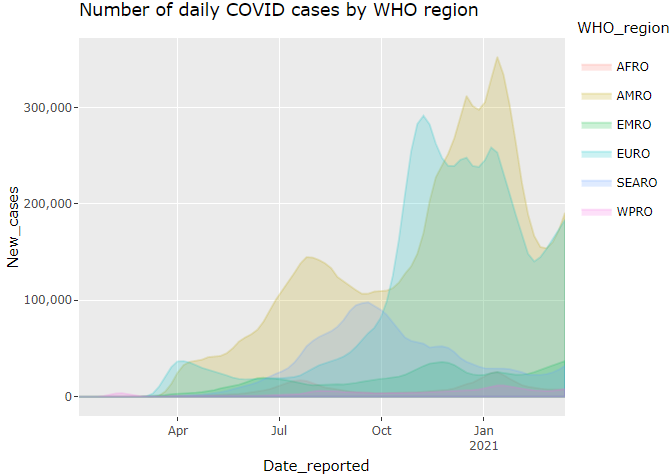
\includegraphics[width=0.8\linewidth]{latexpics/decoratorexample1}

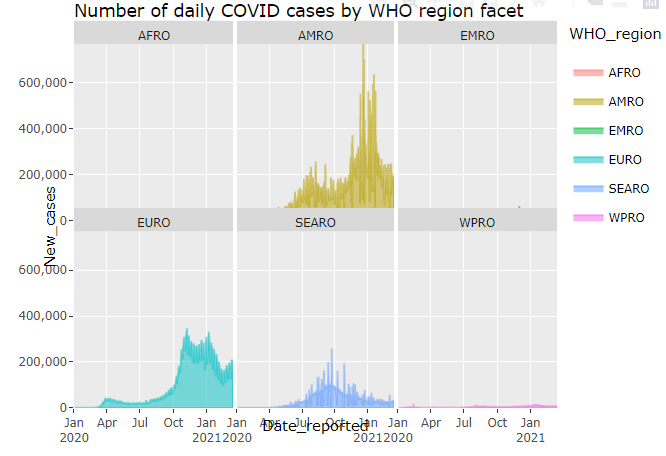
\includegraphics[width=0.8\linewidth]{latexpics/decoratorexample2}

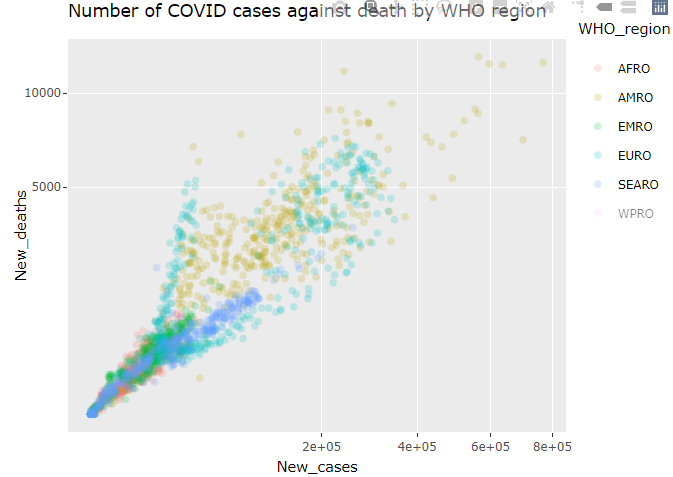
\includegraphics[width=0.8\linewidth]{latexpics/decoratorexample3}

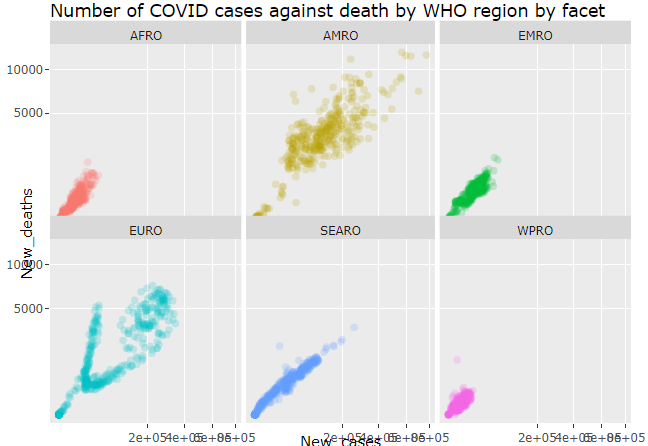
\includegraphics[width=0.8\linewidth]{latexpics/decoratorexample4}

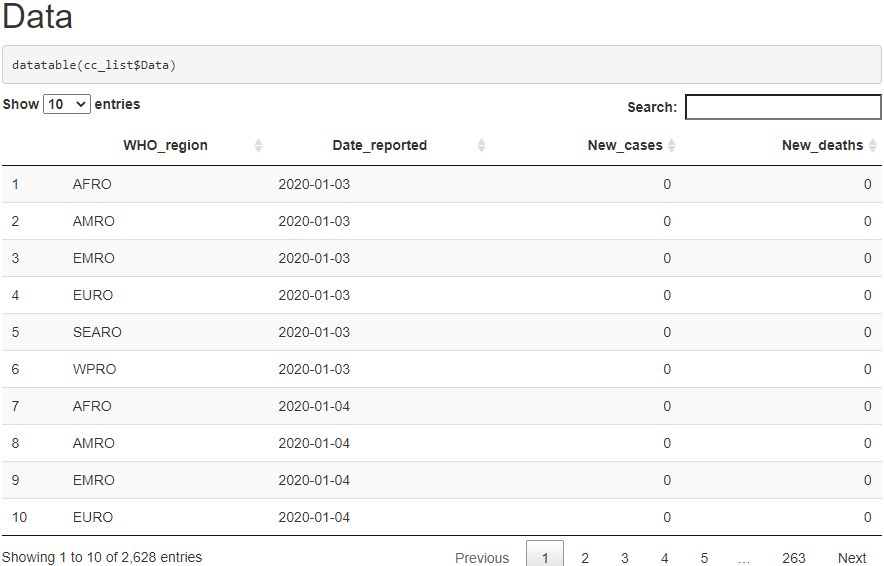
\includegraphics[width=0.8\linewidth]{latexpics/decoratorexample5}

\hypertarget{number-of-new-cases-with-decorators}{%
\subsubsection{Number of New Cases with
decorators}\label{number-of-new-cases-with-decorators}}

After using ggplotly as a decorator method, the exact numbers of new
cases can new be assessed directly in the plotting area. To be general,
only the highest number of new cases from each region with the date
observed will be report. The rest of the information are left with
interest for the readers to interpret and explore. The first set of
plots shows the highest number of new cases in a single day in the given
time frame was 769,644 cases observed from the region of Americas, and
it was the 19th of September 2020. The highest new cases observed in a
single day in the regions of Africa was the 3rd of January, 2021, with
the exact number of 40456. The highest new cases observed in a single
day in the regions of Eastern Mediterranean was the 1st of December,
2020, with the exact number of 62206. The highest new cases observed in
a single day in the regions of European was the 8th of November, 2020,
with the exact number of 346573. The highest new cases observed in a
single day in the regions of South East Asia was the 23th of December,
2020, with the exact number of 78377. Finally, the ``lowest'' region
with highest observed number of new cases in a single day was Western
Pacific region, at the number of 15155, on the 13th of February, 2020.

The number of new cases can not only be interpreted by moving the mouse
pointer over the graphing zone, but also displayed in order by
\emph{Date\_reported} and \emph{New\_cases} in the data table. If the
viewer is looking for observation under specific conditions, such as a
given date, the search function allows direct access within the matching
search. Same from the previous example, the entire webpage with these
features embedded were created using the listdown workflows. No
additional steps were done outside this R markdown document since the
first example.

\hypertarget{number-of-new-cases-and-death-with-decorators}{%
\subsubsection{Number of New Cases and Death with
decorators}\label{number-of-new-cases-and-death-with-decorators}}

The highest number of death and the date observed were also revealed. To
be general, the information will be reported like chapter 3.1.1, rest of
the information are also with interest for the readers to interpret and
explore. In addition from the plot in chapter 2.3.4, the daily highest
number of deaths was from Region of the Americas, with a single day
number of new cases at 565201, the deaths was 12407. To check for the
exact date of this observations, we selected ordering the
\emph{New\_deaths} variable in descending order, and refer to the
\emph{Date\_reported} variable. The date was 22nd of January, 2021.

The linkage use of plotly and datatable revealed this finding in almost
no time. On top of this HTML webpage, it was produced with listdown's
high efficiency workflows. If the task was done without decorators, the
viewers will never see the exact numbers unless scrolling through the
2628 views of observations. Or the author will have to produce the whole
document in a separate normal R markdown workflow saving everything in
its very own directory.

\hypertarget{decorators-for-more-complicated-computational-compontents}{%
\subsection{Decorators for more complicated computational
compontents}\label{decorators-for-more-complicated-computational-compontents}}

The previous example reflected the improvements in visual perception by
using decorators compared to static plots. However, both cases were
considered as basic usage in the prospect of decorator introduction from
On the Programmatic Generation of Reproducible Documents (Kane,Jiang and
Urbanek, 2020). The ggplot takes two main arguments when producing a
plot. First, the source of the data desired to be visualized are stated.
Then the aes() argument maps components of the data set to the
components in a visualization. The computational components from chapter
2.3 contains the plotting mechanism and the actual plots stored as list
type objects. The decorator method, function ggplotly seeks all the
mapping components in the same directory as the ggplot during the
mapping process. However, that is not stated by default in all packages.
The methods described by decorators can sometimes seek mapping
components in different directories, or pathways. If this happens, the
described decorator method inherits the original function in the
computational component, but fails to find the mapping components
required, the decorator method will fail to work and return an error
message indicating the problem. In the next example, we have used
another set of data from the \emph{gapminder} package (Bryan, 2017).
There are two main aspects demonstrated by the following example.
Firstly, as previous examples demonstrated, despite facetting is an
effective visualization method, but when the data set has variables with
a large number of categorical levels, the original function
facet\_wrap() embedded in package ggplot2 may become inefficient. The
package trelliscope (Hafen, Gosink, McDermott, Rodland, Kleese-Van Dam
and Cleveland, 2013) subsets data into groups and facets the plots
arranging each plot in a grid. Although it provides a better solution
compared to facet\_wrap, the second aspect arises when it is used in a
computational component of a listdown object. The method described by
the decorator seeks a different pathway in the mapping process that is
not originally defined by the function in the computational component
from the list.

\hypertarget{visualizing-the-gapminder-data-set}{%
\subsubsection{Visualizing the Gapminder Data
Set}\label{visualizing-the-gapminder-data-set}}

The original data was loaded and added into the list of files. From the
description (Bryan, 2017), the gapminder data set contains information
on the life expectancy, GDP per captia and population of 142 countries
with their continents from 1952 to 2007. In comparison to the case study
from chapter 2.3, the designated facetting variable increased from 6 to
142. We will repeat the listdown workflow process, the RDS file saved
are used in the next chapter for advanced solutions. The chunk of codes
below produces a ggplot with \textbf{facet\_wrap()} using listdown. the
final layout is folded because of too much plots inserted onto the same
panel. The trelliscopejs package(Hafen, Gosink, McDermott, Rodland,
Kleese-Van Dam and Cleveland, 2013) converts ggplot with
\textbf{facet\_wrap()} argument into individual plots with interactive
interface. This package provides us a potential tool expanding each
seperate plot on multiple panels, which will be discussed later in the
paper.

\hypertarget{life-expectancy}{%
\section{life expectancy}\label{life-expectancy}}

From the output shown, simple \textbf{facet\_wrap()} fails to show a
informative visualization. The scales were out of proportion and the
observations were too dense. With the introduction of trelliscopejs, a
solution arises.

\hypertarget{trelliscopejs}{%
\subsubsection{Trelliscopejs}\label{trelliscopejs}}

In the previous writings, trelliscope displays was mentioned several
times as a substitution to facetting functions in ggplot. The idea
behind trelliscope (Becker, Cleveland \& Shyu, 1996) was described as
D\&R, standing for divide and recombine (Guha, Hafen, Rounds, Xia, Li,
Xi, \& Cleveland, 2012) during the development of package
\textbf{trelliscopeJS}. The idea was an approach on methods to display
large complex data visualizations. In a trelliscope system, the data set
are splited into subsets, with a visualization method applied to each
subsets. The output is a structurally arrayed panel each displaying a
portion of the original data (Hafen, Gosink, McDermott, Rodland,
Kleese-Van Dam and Cleveland, 2013). Different from the original
trelliscope displays, once the panel becomes interactive, functions such
as filtering, sorting and searching can be implemented. These derivative
features of an interactive interface provides huge convenience that
static trelliscope displays does not have. To implant this approach into
ggplot2 interface, \textbf{facet\_trelliscope()} was introduced. The
next example shows a simple change in the function solving the problem
in chapter 3.2.1.

\hypertarget{facetting-using-package-trelliscopejs}{%
\subsubsection{Facetting using Package
TrelliscopeJS}\label{facetting-using-package-trelliscopejs}}

After using \textbf{facet\_trelliscope()}, the gapminder data set
returns an visual output much more interpretable than before. However,
this was created in a normal R markdown workflow.

\begin{verbatim}
## using data from the first layer
\end{verbatim}

\begin{verbatim}
## PhantomJS not found. You can install it with webshot::install_phantomjs(). If it is installed, please make sure the phantomjs executable can be found via the PATH variable.
\end{verbatim}

\hypertarget{motivations-of-implementing-trelliscope-into-listdown}{%
\subsubsection{Motivations of implementing Trelliscope into
listdown}\label{motivations-of-implementing-trelliscope-into-listdown}}

There are several reasons trelliscopeJS may be even more efficient when
it is implemented into listdown compared to a normal R markdown output.
Firstly, big data outputs are usually produced with more complicated
computational components. Part of listdown's purpose was to make the
output documents more ``content based'' instead of ``coding and
techniqucal based''. The computational component's output can be
displayed in an more elegant format without excessive code chunk control
options, authors have higher work efficiency when producing trelliscope
in a listdown workflow compared to a normal R markdown workflow.

Secondly, big data visualizations are often presented to a large number
of audience whether it is used for explanatory or predictive analysis.
While the author may save some time producing and creating the
visualizations, it is important for the audience to focus on the
outputs. The interpretation for these multi-panel plots may take up
hours or even days of time before any conclusion can be found for
experts. On the other hand, if trelliscope visualizations are used for
example, in an exhibition or presentation open to public, audience with
little to no statistical knowledge are expected. The standardization of
all computational components, especially graphical outputs helps readers
in capturing key information regardless the targeted occasions. Both
listdown and trelliscopejs packages were created in the common purpose
based on the points mentioned above.

Last but not least, previous studies mentioned the importance of
obtaining full saturated information from big data, specifically in
marketing (Keahey, 2013) and clinical health data (Kane,Jiang and
Urbanek, 2020). One could influence the strategical plan and investment
funds for a company like IBM (Keahey, 2013), the other could find cures
to intractable diseases. Trelliscopejs has the ability to organize all
visualizations and listdown has the ability to organized the
computational components producing the visualizations.

Implementing a trelliscope system into listdown sounds like a staggered
computing task, but listdown has an argument specially designed for
describing the output methods, and this is achieved by modifying the
decorators, demonstrated in chapter 3.1 using plotly. In the next
chapter, several approaches are taken to achieve this goal.

\hypertarget{solution-using-decorators}{%
\section{Solution using Decorators}\label{solution-using-decorators}}

As previous examples demonstrated. The decorator indicates a name of
method or function that are applied to the stated class of object in the
listdown file during kniting process. The goal is to swap
\textbf{facet\_wrap()} with \textbf{facet\_trelliscope()}, and it
requires partially changing the function call of the ggplot object in
listdown. One fast solution was to exclude the \textbf{facet\_wrap()}
function from the listdown file and add \textbf{facet\_trelliscope()}
through \textbf{initial\_expr()} argument. The code chunk in
\textbf{initial\_expr()} is inserted immediately once the required
libraries are loaded. When render is called knitting the listdown
object, codes in \textbf{initial\_expr()} is evaluated before the
listdown objects are rendered. The following example demonstrates this
approach.

\hypertarget{adding-trelliscopejs-facet-for-gapminder-in-listdown}{%
\subsection{Adding trelliscopejs facet for Gapminder in
listdown}\label{adding-trelliscopejs-facet-for-gapminder-in-listdown}}

To exclude the facet argument, we recreated the computational component
with no facet arguments, and save the list into an RDS file named
\emph{comp-comp\_gapminder\_trellis.rds}. Everything else remains the
same within a normal R markdown workflow.

\begin{Shaded}
\begin{Highlighting}[]
\CommentTok{\# Creating the computational components, this time without the \textquotesingle{}facet\_wrap\textquotesingle{} call.}
\KeywordTok{library}\NormalTok{(gapminder)}

\NormalTok{comp\_comp\_gapminder\_trellis \textless{}{-}}\StringTok{ }\KeywordTok{list}\NormalTok{(}
  \StringTok{\textasciigrave{}}\DataTypeTok{life expectancy full}\StringTok{\textasciigrave{}}\NormalTok{ =}\StringTok{ }\KeywordTok{ggplot}\NormalTok{(gapminder) }\OperatorTok{+}\StringTok{ }\KeywordTok{geom\_point}\NormalTok{(}\KeywordTok{aes}\NormalTok{(}\DataTypeTok{x =}\NormalTok{ year, }\DataTypeTok{y =}\NormalTok{ lifeExp)) }\OperatorTok{+}\StringTok{ }
\StringTok{                           }\KeywordTok{xlim}\NormalTok{(}\DecValTok{1948}\NormalTok{, }\DecValTok{2011}\NormalTok{) }\OperatorTok{+}\StringTok{ }\KeywordTok{ylim}\NormalTok{(}\DecValTok{10}\NormalTok{, }\DecValTok{95}\NormalTok{) }\OperatorTok{+}\StringTok{ }\KeywordTok{theme\_bw}\NormalTok{() }\OperatorTok{+}\StringTok{ }
\StringTok{                           }\KeywordTok{labs}\NormalTok{(}\DataTypeTok{title =} \StringTok{"life expectancy by continent"}\NormalTok{))}

\CommentTok{\#Save file to the disk}
 \KeywordTok{saveRDS}\NormalTok{(comp\_comp\_gapminder\_trellis, }\StringTok{"comp{-}comp\_gapminder\_trellis.rds"}\NormalTok{)}
\end{Highlighting}
\end{Shaded}

The new function \textbf{ggtre()} is created in the initial expression.
The function consists of two parts, the first being the original
function call. In this example, it was the ggplot objects in the
listdown file. The second part is the \textbf{facet\_trelliscope()}
arguments with the facetting variables and other parameters. The
additional argument here is the pathway of the function call.
Trelliscope had a bug, it attempts to find the variable attributes with
default, which is NULLdata. By adding a pathway using
\textbf{path=``.''} argument, facet\_trelliscope now changes the pathway
to the current working directory. once knitr is called from rendering
the listdown object, initial expression gets evaluated first. The
decorator method is directed to the right pathway containing the
elements need for the trelliscope argument.

\begin{Shaded}
\begin{Highlighting}[]
\KeywordTok{library}\NormalTok{(listdown)}
\CommentTok{\# Adding trelliscope call in the initial expressions, notice the description: Path ="."}

\NormalTok{ld\_gapminder\_trellis \textless{}{-}}
\StringTok{  }\KeywordTok{listdown}\NormalTok{(}\DataTypeTok{load\_cc\_expr =} \KeywordTok{readRDS}\NormalTok{(}\StringTok{"comp{-}comp\_gapminder\_trellis.rds"}\NormalTok{),}
                \DataTypeTok{package =} \KeywordTok{c}\NormalTok{(}\StringTok{"ggplot2"}\NormalTok{,}\StringTok{"gapminder"}\NormalTok{, }\StringTok{"trelliscopejs"}\NormalTok{),}
              \DataTypeTok{decorator =} \KeywordTok{list}\NormalTok{(}\DataTypeTok{ggplot =}\NormalTok{ ggtre), }
              \DataTypeTok{init\_expr =}\NormalTok{ \{}
\NormalTok{                  ggtre =}\StringTok{ }\ControlFlowTok{function}\NormalTok{(x) x }\OperatorTok{+}
\StringTok{                          }\KeywordTok{facet\_trelliscope}\NormalTok{(}\OperatorTok{\textasciitilde{}}\StringTok{ }\NormalTok{country }\OperatorTok{+}\StringTok{ }\NormalTok{continent,}
                                            \DataTypeTok{nrow =} \DecValTok{2}\NormalTok{, }\DataTypeTok{ncol =} \DecValTok{7}\NormalTok{, }\DataTypeTok{width =} \DecValTok{300}\NormalTok{, }\DataTypeTok{path =} \StringTok{"."}\NormalTok{)}
\NormalTok{                          \})}
\NormalTok{ld\_gapminder\_trellis}
\end{Highlighting}
\end{Shaded}

\begin{verbatim}
## 
## Listdown object description
## 
##     Package(s) imported:
##  ggplot2
##  gapminder
##  trelliscopejs
## 
##     Setup expression(s) (run before packages are loaded):
##  (none)
## 
##     Initial expression(s) (run after packages are loaded):
##  {
##      ggtre = function(x) x + facet_trelliscope(~country + continent, 
##          nrow = 2, ncol = 7, width = 300, path = ".")
##  }
## 
##     Expression to read data:
##  readRDS("comp-comp_gapminder_trellis.rds")
## 
##     Decorator(s):
##  Type    Method
##  ggplot  ggtre
## 
##     Defaut decorator:
##  identity
## 
##     Chunk option(s):
##  (none)
## 
##     Decorator chunk option(s):
##  (none)
\end{verbatim}

From the description of the listdown method above, the initial
expression that gets to run immediately after packages are loaded are
now included. The decorator method for ggplot class objects are now
rendered using the method \textbf{ggtre()} described in the initial
expression. The next chunk of codes follows a normal listdown workflow
and produces the document \emph{gapminder\_trellis-example.html},
implementing trelliscope to ggplot.

\begin{Shaded}
\begin{Highlighting}[]
\KeywordTok{library}\NormalTok{(rmarkdown)}
\NormalTok{gapminder\_trellis\_example \textless{}{-}}\StringTok{ }\KeywordTok{c}\NormalTok{(}
 \KeywordTok{as.character}\NormalTok{(}\KeywordTok{ld\_rmarkdown\_header}\NormalTok{(}\StringTok{"gapminder plots using trelliscope"}\NormalTok{,}
              \DataTypeTok{author =} \StringTok{"Leon"}\NormalTok{, }\DataTypeTok{date =} \StringTok{"2021"}\NormalTok{)), }\KeywordTok{ld\_make\_chunks}\NormalTok{(ld\_gapminder\_trellis))}
\end{Highlighting}
\end{Shaded}

\hypertarget{a-more-generalized-solution}{%
\subsection{A More Generalized
Solution}\label{a-more-generalized-solution}}

Each country can now be shown clearly like the output from a normal R
markdown workflow. Despite this simple and quick approach has reached
the ultimate goal, it has multiple problems that needs to be considered.
Firstly, in this approach, the function in the listdown file was
modified to fit the requirement for using \textbf{ggtre()} added. To be
more exact, we deliberately deleted the \textbf{facet\_wrap()} argument
from the ggplot object ``life expectancy full'' in the list
``comp\_comp\_gapminder\_trellis'' to suit the function in initial
expression. Secondly, the initial expression are passed onto all objects
of the same class within the same listdown file. If there were some
ggplot objects in the listdown file that the author do not wish to
seperate, it is not possible when this function is applied. Thirdly, the
variables in \textbf{ggtre()} are fixed for each listdown file. This
means only the same variables are used in all ggplot objects in a data
set, if there were any ggplot objects which does not have the variable
described in \textbf{ggtre()}, this approach would not work. It was also
suggested the number of initial expression and the complexity of the
initial expression shall be kept minimal (Kane,Jiang and Urbanek, 2020).
The initial expression is considerably long in this case, and could be
even longer if further arguments were added. A more generalized approach
shall be developed.

\hypertarget{facet_wrap-to-facet_trelliscope}{%
\subsection{facet\_wrap to
facet\_trelliscope}\label{facet_wrap-to-facet_trelliscope}}

The common ground for \textbf{facet\_wrap()} and
\textbf{facet\_trelliscope()} is their concept of dividing the data into
smaller subsets and recombine them into either a panel or multiple
arrays of plots. For the two different arguments, the variable used as
the subsetting condition is the same through out the process. If a
function could pull the facetting variables out from
\textbf{facet\_wrap()}, then places it into
\textbf{facet\_trelliscope()}, then we could get rid of the
\textbf{facet\_wrap()} in the function without the need to modify the
original ggplot funtion from listdown. The only problem remains is the
facetting layer left in the old ggplot arguments which needs to be
removed and replaced by the new trelliscope facets. The function
\textbf{facet\_wrap2ts()} was designed to solve the issues mention
above. This solves the problem from chapter 4.1 in a more generalized
way, no modifications needs to be carried out on the original ggplot
function in listdown.

\hypertarget{function-facet_wrap2ts}{%
\subsubsection{Function facet\_wrap2ts}\label{function-facet_wrap2ts}}

The function \textbf{facet\_wrap2ts} designed to be a decorator method
for the listdown package is shown below.

This function works as follows:

\begin{enumerate}
\def\labelenumi{\arabic{enumi}.}
\item
  we assume y is a ggplot class object in the list of objects, and it
  has an argument for facet. The first \textbf{if} statement states that
  facet argument of the ggplot object y must have a facet and must not
  be the class ``facetNULL'', or empty, which means there simply is no
  facet. Then the transformation process is continued.
\item
  Next, a vector v is created, which obtains the variable names from the
  facet argument within the ggplot object y. The variable names in v are
  important because it will be passed to \textbf{facet\_trelliscope()}'s
  facet arguments. We are not changing any variables of the data to
  visualize at this step, but the function of which the variables gets
  fed into.
\item
  Now, because the ggplot object y still has the original layer of facet
  that needs to be replaced by the new trelliscope facet, we created an
  empty ggplot object \textbf{o}. Then the empty facet attribution named
  \emph{facetNULL} in object \textbf{o} gets pulled out.
  \emph{facetNULL} are then injected into the already existing facet
  attributes in y. Up to this step, y still remains to be the exact same
  ggplot object as original, except without the facet argument.
\item
  The formula is then created using the original facet variables
  previously stored in v and the correct syntax. It is converted from an
  R object of the character class to an R object of the expression
  class. Before step 5, it is evaluated and ready to be used to build
  the function call.
\item
  The next step is constructing the function call.
  \textbf{facet\_trelliscope()} argument were implanted with the new
  formula named \emph{form} from the previous steps.
\item
  The last step is to call the original ggplot object y combined with
  the evaluated result of the new function \textbf{c}. This returns an
  output that shall look identical to using
  \textbf{facet\_trelliscope()} in normal R markdown files.
\item
  There are also cases this decorator is applied improperly, for example
  when the ggplot object y does not contain any facet arguments, that is
  the attribute being facetNULL. This is encountered by using the
  \textbf{else} from the if loop. The output remains the exact same of y
  untouched. If users intend to add a \textbf{facet\_wrap()} as a
  decorator, then function style \textbf{ggtre} can be used. It requires
  the user to manually set the variables for facetting, and the
  decorator function shall be included as an intial expression, which
  gets evaluated before the knitting process.
\end{enumerate}

\hypertarget{testing-facet_wrap2ts-on-gapminder-data-set}{%
\subsubsection{Testing facet\_wrap2ts on Gapminder Data
set}\label{testing-facet_wrap2ts-on-gapminder-data-set}}

To testify if the function works for the gapminder data set, the same
listdown object was used from chapter 3.2.1. This time, the initial
expression was removed, and the decorator was changed to the new
function. The listdown object was saved as
\emph{ld\_gapminder\_trellis\_generic}. After adding the headers, we
rendered the document to check the outputs.

\begin{Shaded}
\begin{Highlighting}[]
\CommentTok{\#\# Same data set as the first example, switching the decorator this time instead of adding initial expression}
\NormalTok{ld\_gapminder\_trellis\_generic \textless{}{-}}
\StringTok{  }\KeywordTok{listdown}\NormalTok{(}\DataTypeTok{load\_cc\_expr =} \KeywordTok{readRDS}\NormalTok{(}\StringTok{"comp{-}comp\_gapminder.rds"}\NormalTok{),}
                \DataTypeTok{package =} \KeywordTok{c}\NormalTok{(}\StringTok{"ggplot2"}\NormalTok{,}\StringTok{"gapminder"}\NormalTok{, }\StringTok{"trelliscopejs"}\NormalTok{),}
              \DataTypeTok{decorator =} \KeywordTok{list}\NormalTok{(}\DataTypeTok{ggplot =}\NormalTok{ facet\_wrap2ts)}
\NormalTok{  )}

\NormalTok{gapminder\_trellis\_generic\_example \textless{}{-}}\StringTok{ }\KeywordTok{c}\NormalTok{(}
 \KeywordTok{as.character}\NormalTok{(}\KeywordTok{ld\_rmarkdown\_header}\NormalTok{(}\StringTok{"gapminder plots trelliscope generic"}\NormalTok{,}
              \DataTypeTok{author =} \StringTok{"Leon"}\NormalTok{, }\DataTypeTok{date =} \StringTok{"2021"}\NormalTok{)), }\KeywordTok{ld\_make\_chunks}\NormalTok{(ld\_gapminder\_trellis\_generic))}

\NormalTok{ld\_gapminder\_trellis\_generic}
\end{Highlighting}
\end{Shaded}

\begin{verbatim}
## 
## Listdown object description
## 
##     Package(s) imported:
##  ggplot2
##  gapminder
##  trelliscopejs
## 
##     Setup expression(s) (run before packages are loaded):
##  (none)
## 
##     Initial expression(s) (run after packages are loaded):
##  (none)
## 
##     Expression to read data:
##  readRDS("comp-comp_gapminder.rds")
## 
##     Decorator(s):
##  Type    Method
##  ggplot  facet_wrap2ts
## 
##     Defaut decorator:
##  identity
## 
##     Chunk option(s):
##  (none)
## 
##     Decorator chunk option(s):
##  (none)
\end{verbatim}

After applying the \textbf{facet\_wrap2ts} decorator function, the
rendering showed a promising result of the HTML document. This concept
can be further extended and used on more decorators for the listdown
package.

\hypertarget{facet_wrap-directly-to-facet_trelliscope-with-plotly}{%
\subsection{facet\_wrap directly to facet\_trelliscope with
plotly}\label{facet_wrap-directly-to-facet_trelliscope-with-plotly}}

The \textbf{facet\_wrap2ts} was successful in turning ggplot objects
with facet argument into trelliscope plots in listdown. However, during
big data set visualizations, we saw the power of ggplotly as a decorator
from example 3.1. It would be appropriate to combine library plotly with
trelliscope, and implement it into a listdown decorator. This fulfills
the needs of decorators when users produce documents via a listdown
workflow that is intended for big data visualizations. From the original
trelliscope package, plotly was supported as one of the arguments in
function \textbf{facet\_trelliscope()}. If we added the arguments and
set the default \textbf{as\_plotly = TRUE}, the output shall be
interactive, while the layout remains the same of using trelliscope.

\hypertarget{function-facet_tsplotly}{%
\subsubsection{Function facet\_tsplotly}\label{function-facet_tsplotly}}

The function \textbf{facet\_tsplotly} was created based on
\textbf{facet\_wrap2ts}. The majority of workflow remains identical
except during the function call constructing step. The extra argument
\textbf{as\_plotly} was fed into the function call during the call
construction process, and gets evaluated with the new call. As with the
same that if p does not have a facet, then the ggplot object would
remain untouched.

\hypertarget{testing-facet_tsplotly-on-gapminder-data-set}{%
\subsubsection{Testing facet\_tsplotly on Gapminder Data
set}\label{testing-facet_tsplotly-on-gapminder-data-set}}

To testify if the decorator method is working. Again, the RDS file
created for the gapminder data set from chapter 3.2.1 will be used. The
decorator in the newly created listown object
\emph{ld\_gapminder\_trellis\_plotly} was changed to
\textbf{facet\_tsplotly} this time.

\begin{Shaded}
\begin{Highlighting}[]
\KeywordTok{library}\NormalTok{(plotly)}

\CommentTok{\#\# Still the same data set as the first example}
\NormalTok{ld\_gapminder\_trellis\_plotly \textless{}{-}}
\StringTok{  }\KeywordTok{listdown}\NormalTok{(}\DataTypeTok{load\_cc\_expr =} \KeywordTok{readRDS}\NormalTok{(}\StringTok{"comp{-}comp\_gapminder.rds"}\NormalTok{),}
                \DataTypeTok{package =} \KeywordTok{c}\NormalTok{(}\StringTok{"ggplot2"}\NormalTok{,}\StringTok{"gapminder"}\NormalTok{, }\StringTok{"trelliscopejs"}\NormalTok{, }\StringTok{"plotly"}\NormalTok{),}
              \DataTypeTok{decorator =} \KeywordTok{list}\NormalTok{(}\DataTypeTok{ggplot =}\NormalTok{ facet\_tsplotly)}
\NormalTok{)}

\NormalTok{gapminder\_trellis\_plotly\_example \textless{}{-}}\StringTok{ }\KeywordTok{c}\NormalTok{(}
 \KeywordTok{as.character}\NormalTok{(}\KeywordTok{ld\_rmarkdown\_header}\NormalTok{(}\StringTok{"gapminder plots trelliscope plotly"}\NormalTok{,}
              \DataTypeTok{author =} \StringTok{"Leon"}\NormalTok{, }\DataTypeTok{date =} \StringTok{"2021"}\NormalTok{)), }\KeywordTok{ld\_make\_chunks}\NormalTok{(ld\_gapminder\_trellis\_plotly))}
\NormalTok{ld\_gapminder\_trellis\_plotly}
\end{Highlighting}
\end{Shaded}

\begin{verbatim}
## 
## Listdown object description
## 
##     Package(s) imported:
##  ggplot2
##  gapminder
##  trelliscopejs
##  plotly
## 
##     Setup expression(s) (run before packages are loaded):
##  (none)
## 
##     Initial expression(s) (run after packages are loaded):
##  (none)
## 
##     Expression to read data:
##  readRDS("comp-comp_gapminder.rds")
## 
##     Decorator(s):
##  Type    Method
##  ggplot  facet_tsplotly
## 
##     Defaut decorator:
##  identity
## 
##     Chunk option(s):
##  (none)
## 
##     Decorator chunk option(s):
##  (none)
\end{verbatim}

The output was interactive. Each individual observations for each
country was interactive. Improving the power of the overall
visualization.

\hypertarget{decorator-application-reporting-number-of-new-cases-and-death-information-from-covid-data}{%
\section{Decorator Application: Reporting number of new cases and Death
information from COVID
Data}\label{decorator-application-reporting-number-of-new-cases-and-death-information-from-covid-data}}

\#@ The Data Set From the previous chapters, the trelliscope works
especially well with big data set having variables with multiple levels.
The plotly interactive plots showed more details on each individual
plots. The decorator function combining the two methods was created and
testified. In this chapter, lets go back to the full COVID-19 data. The
data set was sourced from World Health Organization official website.
All data was provided to the date before this paper was completely
finished. Based on the description
(\url{https://covid19.who.int/info/)The} full data set contains the
following information:

\begin{itemize}
\tightlist
\item
  Date\_reported
\end{itemize}

The date reported variable was in the class type of dates. The variable
records the date of the information reported to WHO.

\begin{itemize}
\tightlist
\item
  Country\_code
\end{itemize}

The Country code variable is the ISO (International Organization for
Standardization) Alpha-2 coundtry codes. The column was recorded with
character strings.

\begin{itemize}
\tightlist
\item
  Country
\end{itemize}

The Country variable contains the names of all the WHO membership
countries, some names aslo stands for political regions or areas if not
claimed to be a country. The column type is also character string class.

\begin{itemize}
\tightlist
\item
  WHO\_region
\end{itemize}

The WHO region variable was previously introduced back in the first case
study. The six big WHO regions are: African Region, Region of the
Americas, South-East Asia Region, European Region, Eastern Mediterranean
Region, and Western Pacific Region. This column is also a character
string class, the column recorded the abbreviations of the regions
instead of the full names.

\begin{itemize}
\tightlist
\item
  New\_cases
\end{itemize}

The new cases variable records the number of new confirmed cases each
day by subtracting previous cumulative case count from current
cumulative cases count from WHO. The column was recorded in the class
integers.

\begin{itemize}
\tightlist
\item
  Cumulative\_cases
\end{itemize}

The cumulative cases records the confirmed cases reported to WHO up to
the date in date reported. The column was in the integer string class.

\begin{itemize}
\tightlist
\item
  New\_deaths
\end{itemize}

The new deaths variable records the new confirmed deaths each day. The
calculation methods were the same as recording the new cases number and
is recorded as integer class.

\begin{itemize}
\tightlist
\item
  Cumulative\_deaths
\end{itemize}

The cumulative deaths number was recorded the same as the cumulative
cases number, and is recorded as the integer class.

As the data was obtained from WHO in raw csv files, a few data cleaning
and tidying were required before plotting. The overall process was
smooth as the quality of the data was very high.

\hypertarget{applying-the-decorator}{%
\subsection{Applying the decorator}\label{applying-the-decorator}}

In this case study, we created a new list named
``comp\_comp\_covid\_trellis''. This list contains the data and the
ggplot object with a facet variable of countries, the interest in this
study was the difference in number of new cases by each different
country. After the list was created ad stored as RDS file, the listdown
object \emph{ld\_covid\_trellis} was created. The decorators in this
listdown object are:

\begin{itemize}
\tightlist
\item
  Method \textbf{datatable} were used instead of data.frame for showing
  the data set.
\item
  Method \textbf{facet\_tsplotly} were used in all ggplot class objects
  for plotting.
\end{itemize}

A full header was then added, the final HTML document
\emph{covid\_trellis-example.html} was rendered and included below.

\begin{Shaded}
\begin{Highlighting}[]
\KeywordTok{library}\NormalTok{(trelliscopejs)}
\KeywordTok{library}\NormalTok{(listdown)}
\KeywordTok{library}\NormalTok{(tidyverse)}
\KeywordTok{library}\NormalTok{(rmarkdown)}
\CommentTok{\#Reading in the data}
\NormalTok{covidcountries \textless{}{-}}\StringTok{ }\KeywordTok{read.csv}\NormalTok{(}\StringTok{"WHO{-}COVID{-}19{-}global{-}data.csv"}\NormalTok{,}
                     \DataTypeTok{colClasses=}\KeywordTok{c}\NormalTok{(}\StringTok{"Date"}\NormalTok{, }\KeywordTok{rep}\NormalTok{(}\StringTok{"character"}\NormalTok{, }\DecValTok{3}\NormalTok{), }
                                   \KeywordTok{rep}\NormalTok{(}\StringTok{"numeric"}\NormalTok{, }\DecValTok{4}\NormalTok{))) }
\KeywordTok{names}\NormalTok{(covidcountries)[}\DecValTok{1}\NormalTok{] \textless{}{-}}\StringTok{ "Date\_reported"}

\CommentTok{\# Creating the list}
\NormalTok{comp\_comp\_covid\_trellis \textless{}{-}}\StringTok{ }\KeywordTok{list}\NormalTok{(}
  \DataTypeTok{Data =}\NormalTok{ covidcountries,}
  \StringTok{\textasciigrave{}}\DataTypeTok{New COVID{-}19 details per day for each Country}\StringTok{\textasciigrave{}}\NormalTok{ =}\StringTok{ }\KeywordTok{ggplot}\NormalTok{(covidcountries) }\OperatorTok{+}
\StringTok{    }\KeywordTok{geom\_point}\NormalTok{(}\KeywordTok{aes}\NormalTok{(}\DataTypeTok{x=}\NormalTok{Date\_reported, }\DataTypeTok{y=}\NormalTok{New\_cases, }\DataTypeTok{group=}\NormalTok{Country), }\DataTypeTok{size =} \FloatTok{0.6}\NormalTok{) }\OperatorTok{+}\StringTok{ }
\StringTok{    }\KeywordTok{geom\_line}\NormalTok{(}\KeywordTok{aes}\NormalTok{(}\DataTypeTok{x=}\NormalTok{Date\_reported, }\DataTypeTok{y=}\NormalTok{New\_cases, }\DataTypeTok{group=}\NormalTok{Country), }\DataTypeTok{size =} \FloatTok{0.4}\NormalTok{) }\OperatorTok{+}
\StringTok{    }\KeywordTok{scale\_x\_date}\NormalTok{(}\DataTypeTok{date\_breaks =} \StringTok{"3 month"}\NormalTok{, }\DataTypeTok{date\_labels =}  \StringTok{"\%b \%Y"}\NormalTok{) }\OperatorTok{+}
\StringTok{    }\KeywordTok{theme\_bw}\NormalTok{() }\OperatorTok{+}
\StringTok{    }\KeywordTok{labs}\NormalTok{(}\DataTypeTok{title =} \StringTok{"COVID{-}19 Details by Country"}\NormalTok{) }\OperatorTok{+}\StringTok{ }
\StringTok{    }\KeywordTok{facet\_wrap}\NormalTok{(}\KeywordTok{vars}\NormalTok{(Country))}
\NormalTok{  )}

\CommentTok{\#Save file to the disk}
\KeywordTok{saveRDS}\NormalTok{(comp\_comp\_covid\_trellis, }\StringTok{"comp{-}comp\_covid\_trellis.rds"}\NormalTok{)}
 
\CommentTok{\# Creating the listdown object}
\NormalTok{ld\_covid\_trellis \textless{}{-}}
\StringTok{  }\KeywordTok{listdown}\NormalTok{(}\DataTypeTok{load\_cc\_expr =} \KeywordTok{readRDS}\NormalTok{(}\StringTok{"comp{-}comp\_covid\_trellis.rds"}\NormalTok{),}
                \DataTypeTok{package =} \KeywordTok{c}\NormalTok{(}\StringTok{"ggplot2"}\NormalTok{,}\StringTok{"trelliscopejs"}\NormalTok{, }\StringTok{"DT"}\NormalTok{),}
              \DataTypeTok{decorator =} \KeywordTok{list}\NormalTok{(}\DataTypeTok{ggplot =}\NormalTok{ facet\_tsplotly, }
                               \DataTypeTok{data.frame =}\NormalTok{ datatable)}
\NormalTok{)}

\CommentTok{\# Adding a header}
\NormalTok{covid\_trellis\_example \textless{}{-}}\StringTok{ }\KeywordTok{c}\NormalTok{(}
 \KeywordTok{as.character}\NormalTok{(}\KeywordTok{ld\_rmarkdown\_header}\NormalTok{(}\StringTok{"Covid plots using trelliscopeJS"}\NormalTok{, }\DataTypeTok{author =} \StringTok{"Leon"}\NormalTok{,}
              \DataTypeTok{date =} \StringTok{"2021"}\NormalTok{)), }\KeywordTok{ld\_make\_chunks}\NormalTok{(ld\_covid\_trellis))}
\end{Highlighting}
\end{Shaded}

\hypertarget{discussion}{%
\subsection{Discussion}\label{discussion}}

From the embedded HTML document rendered from chapter 5.2, several
features were included as are discussed below.

\hypertarget{the-data-table}{%
\subsubsection{The Data Table}\label{the-data-table}}

From results provided by the interactive data table, there are over
120,000 rows of observations in total. If this data was displayed using
the original data.frame method, it would be insufficient for readers
scrolling through all of them before any other analytical graphics can
be displayed. On top of the much tidied interface, the observations are
ordered primarily by the alphabetical order of country names, then by
the data reported in the given time frame. For country names that starts
in the middle, the search bar feature provides an alternative approach
rather than scrolling though the entries. These changes can save a huge
amount of time for authors and provides an user-friendly interface for
viewers. The data table interface even works better with the
visualization using trelliscope system following up. The capture below
is a screen shot from the original HTML document. Please refer to the
HTML embedded data table for it's corresponding interactive version.

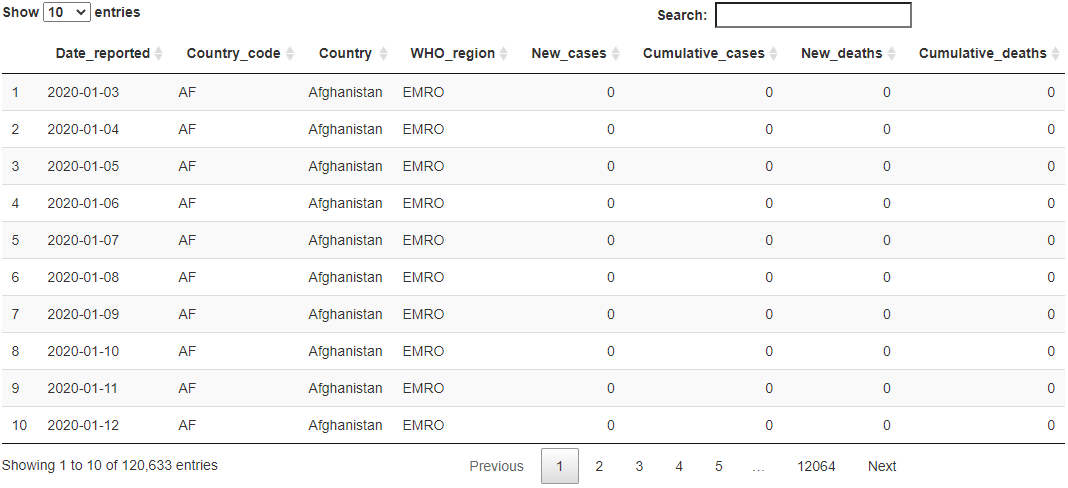
\includegraphics[width=1\linewidth,height=1\textheight]{datatable}

\hypertarget{the-visualization}{%
\subsubsection{The Visualization}\label{the-visualization}}

The final result of the visualization had a elegant and neat layout
compared to all of the previous examples. The data for this case study
was also much bigger compared to previous examples. For the
interpretations of each country, some representative findings are
discussed in this section while the rest are left for the viewers of the
paper to explore. Interpretations are followed in the alphabetical order
of the country names, the display are captured as screen shots for the
purpose of this paper, hence they are not interactive. Please refer to
the trelliscope system for their corresponding interactive counterparts.

\begin{itemize}
\tightlist
\item
  China
\end{itemize}

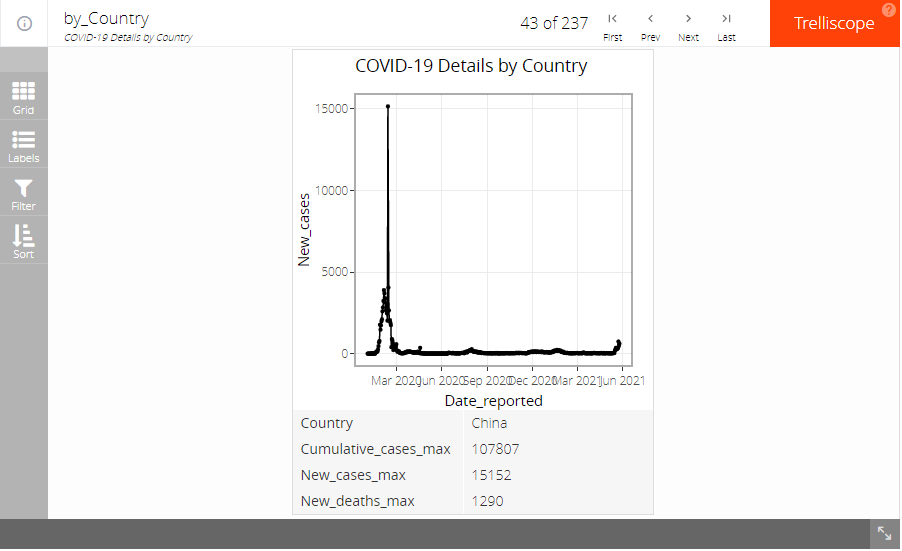
\includegraphics[width=1\linewidth,height=1\textheight]{China}

From the plot of China, where the COVID-19 was first discovered to have
symptoms on humans initially, the rise of number of new cases was rapid
and severe. The single day peak number of new cases discovered was on
the 13th of February, 2020, at 15152 new cases. While this
``outlier-like'' single day number was discrepant to the number provided
from the Wikipedia page of Statistics of the COVID-19 pandemic in
mainland China (\url{https://en.wikipedia.org}), it was then discovered
accordingly to the National Health Commission
(\url{http://en.nhc.gov.cn/}) the previous records of new cases was not
completely recorded and was justified and added on in this particular
day before reporting to WHO. Then China has effectively lowered the
number of new cases daily with a series of actions. However, up to the
date before this paper was finalized, there is a rebound trend, with 743
new cases daily recorded on the 23rd of May, 2021. The time frame of the
peak number and the rebounding trend would have not been noticed without
individual plotting.

\begin{itemize}
\tightlist
\item
  India
\end{itemize}

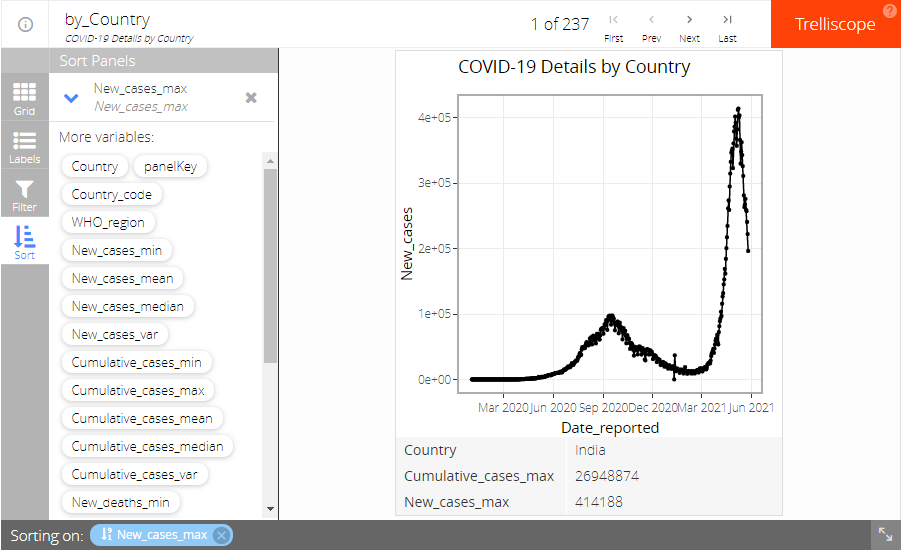
\includegraphics[width=1\linewidth,height=1\textheight]{India}

To Find the plot of India, the sorting feature of trelliscope was
applied. The main interest of India was the daily number of new cases
increases out of control lately. The trend was clearly displayed in the
plot, and reached a peak of 414188 cases on the 7th of May, 2021.
However, if the overall tend was not plotted, a small rise in the number
of new cases has occurred during September, 2020. The daily number of
new cases in India has gained focus worldwide, several medias has
criticized India's continuous poor action and policy decisions, little
knowing the decrease in new cases between October 2020 till March 2021.

\begin{itemize}
\tightlist
\item
  The United States of America
\end{itemize}

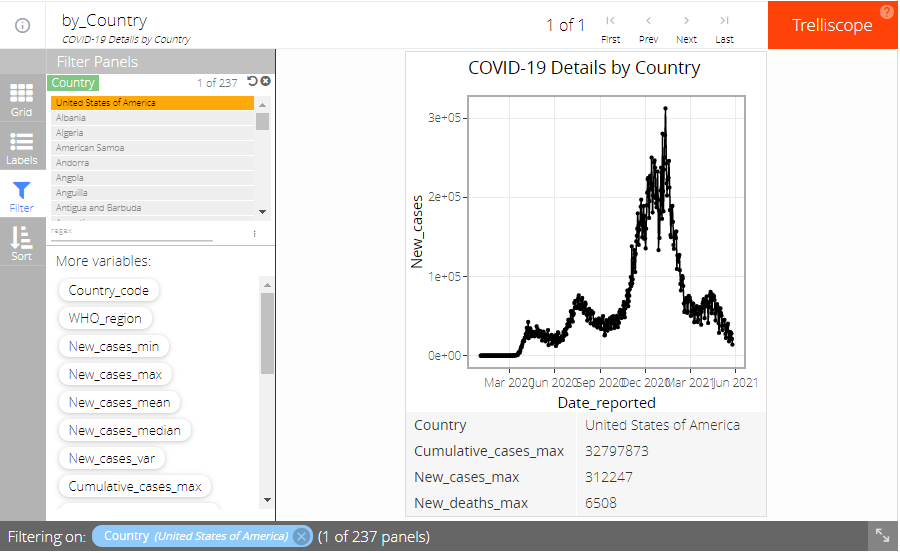
\includegraphics[width=1\linewidth,height=1\textheight]{UnitedStatesofAmerica}

Because United States of America was behind in the alphabetical order of
countries, it is displayed using the filter feature in trelliscope. The
filter feature works like the search feature in data table, instead of
browsing through the countries, users can be navigated to the
visualization from conditions selected in the filtering tab directly.
The other details of interest are also visible below the graphing area,
such as the highest deaths number recorded daily. The U.S. shows a
cyclical behavior in the number of new cases, and had the highest new
cases number 312247 recorded on the 10th of January, 2021.

\begin{itemize}
\tightlist
\item
  Germany and Spain
\end{itemize}

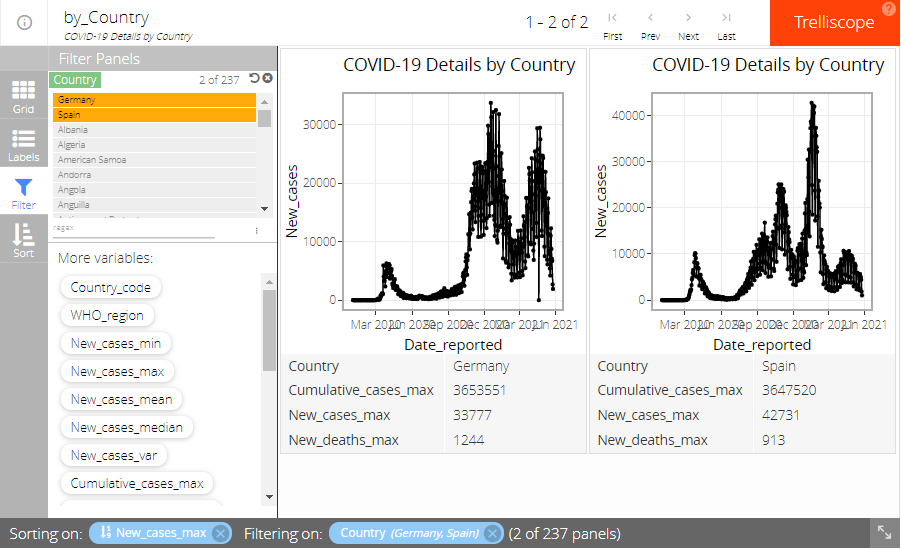
\includegraphics[width=1\linewidth,height=1\textheight]{GermanyvsSpain}

It is also possible to make comparisons between two countries
individually. This plot was made possible by using the customizable grid
option. Users can select displaying multiple columns and rows in the
same graphing zone, and each zone's displaying information can be
selected individually using the filter conditions. The two countries
shown, Germany and Spain are not only closely located geographically,
but also had very similar cumulative new cases number. However, the
trend and pattern of new cases across the same time frame were very
different. The combination of the trelliscope features shown in this
visualization is particularly useful for comparison and exploratory
analyses. On top of the comparison capabilities, the date and new case
numbers for each point of interest are revealed. The plotly tool bars
also allows zooming into a portion of the data for much detailed
interpretation, or users can choose to view the overall system in full
screen allowing for non-overlapping x and y axis scaling.

\hypertarget{conclusion-and-further-work}{%
\section{Conclusion and Further
Work}\label{conclusion-and-further-work}}

\hypertarget{conclusion}{%
\subsection{Conclusion}\label{conclusion}}

In a typical statistical task, the listdown package has great advantage
of more efficient and optimal workflow compared to normal workflows,
especially with the combination of trelliscopejs package. COVID-19 were
one of the diseases that caused a huge impact in the vast era of
mankind. The data and insights obtained worldwide provides precious
experience and shall be presented with the rightful tools. The
trelliscope system combined with listdown package has successfully
demonstrated it's power in this scenario. All of these would not have
been achievable without decorators.

While the advantage of such combination demonstrated easiness in several
aspects on both the author's prospect and the interpreter's prospect, it
shall be kept in mind of when this tool can be deployed appropriately.

For occasions whereas detailed quantitative tasks are carried out, a
full analytical process used in statistics must be required. The steps
often includes but are not limited to hypotheses setting, statistical
testing, assumption checking, executive summary, technical summary,
discussion and conclusions. Most of the steps require narrative
components. Visualization can be applied to some of these steps as
either the final output or used as an assistance, but it will never be
sufficient enough being the only result for all the tasks. In fact,
computational components itself may not be effective on completing a
qualitative statistical task alone (Kane,Jiang and Urbanek, 2020). On
the other hand, despite narrative components can be included into
listdown as character elements using the chunk options decorator by
setting the \textbf{results = ``as.is''}, it contraries the intention of
the authors whom originally created the listdown package, and are
considered less efficient in comparison to using a normal R markdown
workflow.

In situations whereas visualizations are crucial for reaching the goal,
or the targeted audience are much more broader than statistical experts
or professional researchers, these computational components and the
decorators works flawlessly in the listdown package, providing an
effective and powerful tool for data visualizations.

\hypertarget{further-work}{%
\subsection{Further Work}\label{further-work}}

While the decorators now works with trelliscope and plotly, there are
still some issues that is yet to be solved. Firstly, if there are more
than one ggplot objects in a list, both function \textbf{facet\_wrap2ts}
and \textbf{facettsplotly} only supports turning the first ggplot object
into the desired output. This was a problem with the \textbf{path}
argument as trelliscope facet components are stored in different
directories than \textbf{facet\_wrap}. A potential solution could be
creating a structured file directory for the different trelliscope
displays needed in a listdown file. Secondly, The are much more
interactive visualization packages that are potentially possible to
embed to listdown with decorators, such as the \textbf{NetworkD3}
package (Allaire, Ellis, Gandrud, Kuo, Lewis, Owen, et al., 2017). The
ideas from the trelliscope decorators in this paper has provided a
pathway to creating future decorator functions. Furtherwork could focus
on making multiple objects suitable for applying the trellicope
decorators in the same list and creating more decorators for the
\textbf{listdown} package.

Keeping the above discussions in mind, the listdown package with a
powerful visualization decorator will have much wider usage scenarios
and higher popularity in the age of big data.

\hypertarget{appendix}{%
\section*{Appendix}\label{appendix}}
\addcontentsline{toc}{section}{Appendix}

\hypertarget{packages}{%
\subsection{Packages}\label{packages}}

\hypertarget{covid-19-examples}{%
\subsection{COVID-19 Examples}\label{covid-19-examples}}

\begin{verbatim}
## 
## comp_covid
##   |-- New cases per day for each region
##   |  o-- object of type(s):gg ggplot
##   |-- New cases per day for each region facet
##   |  o-- object of type(s):gg ggplot
##   |-- Cases against Death
##   |  o-- object of type(s):gg ggplot
##   o-- Cases against Death facet
##      o-- object of type(s):gg ggplot
\end{verbatim}

\begin{verbatim}
## [1] "listdown"
\end{verbatim}

\begin{verbatim}
## 
## Listdown object description
## 
##     Package(s) imported:
##  ggplot2
##  tidyverse
##  scales
## 
##     Setup expression(s) (run before packages are loaded):
##  (none)
## 
##     Initial expression(s) (run after packages are loaded):
##  (none)
## 
##     Expression to read data:
##  readRDS("comp-comp_covid.rds")
## 
##     Decorator(s):
##  (none)
## 
##     Defaut decorator:
##  identity
## 
##     Chunk option(s):
##  (none)
## 
##     Decorator chunk option(s):
##  (none)
\end{verbatim}

\begin{verbatim}
##  [1] "---"                                              
##  [2] "title: Covid plots"                               
##  [3] "author: Leon"                                     
##  [4] "date: '2021'"                                     
##  [5] "output: html_document"                            
##  [6] "---"                                              
##  [7] ""                                                 
##  [8] "```{r}"                                           
##  [9] "library(ggplot2)"                                 
## [10] "library(tidyverse)"                               
## [11] "library(scales)"                                  
## [12] ""                                                 
## [13] "cc_list <- readRDS(\"comp-comp_covid.rds\")"      
## [14] "```"                                              
## [15] ""                                                 
## [16] "# New cases per day for each region"              
## [17] ""                                                 
## [18] "```{r}"                                           
## [19] "cc_list$`New cases per day for each region`"      
## [20] "```"                                              
## [21] ""                                                 
## [22] "# New cases per day for each region facet"        
## [23] ""                                                 
## [24] "```{r}"                                           
## [25] "cc_list$`New cases per day for each region facet`"
## [26] "```"                                              
## [27] ""                                                 
## [28] "# Cases against Death"                            
## [29] ""                                                 
## [30] "```{r}"                                           
## [31] "cc_list$`Cases against Death`"                    
## [32] "```"                                              
## [33] ""                                                 
## [34] "# Cases against Death facet"                      
## [35] ""                                                 
## [36] "```{r}"                                           
## [37] "cc_list$`Cases against Death facet`"              
## [38] "```"
\end{verbatim}

\hypertarget{covid-19-decorator-examples}{%
\subsection{COVID-19 Decorator
Examples}\label{covid-19-decorator-examples}}

\begin{verbatim}
## 
## Listdown object description
## 
##     Package(s) imported:
##  ggplot2
##  tidyverse
##  scales
##  DT
##  plotly
## 
##     Setup expression(s) (run before packages are loaded):
##  (none)
## 
##     Initial expression(s) (run after packages are loaded):
##  (none)
## 
##     Expression to read data:
##  readRDS("comp-comp_covid.rds")
## 
##     Decorator(s):
##  Type        Method
##  ggplot      ggplotly
##  data.frame  datatable
## 
##     Defaut decorator:
##  identity
## 
##     Chunk option(s):
##  (none)
## 
##     Decorator chunk option(s):
##  (none)
\end{verbatim}

Gapminder Examples

\hypertarget{gapminder-using-trelliscope}{%
\subsection{Gapminder using
Trelliscope}\label{gapminder-using-trelliscope}}

\begin{verbatim}
## using data from the first layer
\end{verbatim}

\hypertarget{solution-using-function-ggtre}{%
\subsection{\texorpdfstring{Solution Using function
\textbf{ggtre}}{Solution Using function ggtre}}\label{solution-using-function-ggtre}}

\begin{verbatim}
## 
## Listdown object description
## 
##     Package(s) imported:
##  ggplot2
##  gapminder
##  trelliscopejs
## 
##     Setup expression(s) (run before packages are loaded):
##  (none)
## 
##     Initial expression(s) (run after packages are loaded):
##  {
##      ggtre = function(x) x + facet_trelliscope(~country + continent, 
##          nrow = 2, ncol = 7, width = 300, path = ".")
##  }
## 
##     Expression to read data:
##  readRDS("comp-comp_gapminder_trellis.rds")
## 
##     Decorator(s):
##  Type    Method
##  ggplot  ggtre
## 
##     Defaut decorator:
##  identity
## 
##     Chunk option(s):
##  (none)
## 
##     Decorator chunk option(s):
##  (none)
\end{verbatim}

\hypertarget{function-facet_wrap2ts-1}{%
\subsection{\texorpdfstring{Function
\textbf{facet\_wrap2ts}}{Function facet\_wrap2ts}}\label{function-facet_wrap2ts-1}}

\begin{verbatim}
## 
## Listdown object description
## 
##     Package(s) imported:
##  ggplot2
##  gapminder
##  trelliscopejs
## 
##     Setup expression(s) (run before packages are loaded):
##  (none)
## 
##     Initial expression(s) (run after packages are loaded):
##  (none)
## 
##     Expression to read data:
##  readRDS("comp-comp_gapminder.rds")
## 
##     Decorator(s):
##  Type    Method
##  ggplot  facet_wrap2ts
## 
##     Defaut decorator:
##  identity
## 
##     Chunk option(s):
##  (none)
## 
##     Decorator chunk option(s):
##  (none)
\end{verbatim}

\hypertarget{function-facet_tsplotly-1}{%
\subsection{Function facet\_tsplotly}\label{function-facet_tsplotly-1}}

\begin{verbatim}
## 
## Listdown object description
## 
##     Package(s) imported:
##  ggplot2
##  gapminder
##  trelliscopejs
##  plotly
## 
##     Setup expression(s) (run before packages are loaded):
##  (none)
## 
##     Initial expression(s) (run after packages are loaded):
##  (none)
## 
##     Expression to read data:
##  readRDS("comp-comp_gapminder.rds")
## 
##     Decorator(s):
##  Type    Method
##  ggplot  facet_tsplotly
## 
##     Defaut decorator:
##  identity
## 
##     Chunk option(s):
##  (none)
## 
##     Decorator chunk option(s):
##  (none)
\end{verbatim}

\hypertarget{covid-19-case-study}{%
\subsection{COVID-19 Case Study}\label{covid-19-case-study}}

\end{document}
